
\documentclass{sig-alternate}

\usepackage{amssymb}
\usepackage{verbatim}
\usepackage{times}
\usepackage{graphicx}
\usepackage{url}
\usepackage{xspace}
\usepackage{float}
\usepackage{latexsym}
\usepackage{natbib}
\usepackage{alltt}
\usepackage{color}
\usepackage{textcomp}
\usepackage{balance}

\bibpunct{[}{]}{,}{n}{}{}

\newcommand{\ie}{\textit{i.e.,} }
\newcommand{\eg}{\textit{e.g.,} }

\def\denseitems{
  \itemsep1pt plus1pt minus1pt
  \parsep0pt plus0pt
  \parskip0pt\topsep0pt}

\begin{document}

\conferenceinfo{FOSE}{'14, May 31 -- June 7, 2014, Hyderabad, India}
\CopyrightYear{2014}
\crdata{978-1-4503-2865-4/14/05}

\title{Software Services: A Research Roadmap}

\numberofauthors{4}

\author{
\alignauthor Satish Chandra\titlenote{\small This author was formerly at IBM.}\\
       \affaddr{Samsung Electronics}\\
       \affaddr{San Jose, CA, USA}\\
       \email{schandra@acm.org}
\alignauthor Vibha Singhal Sinha\\
	\affaddr{IBM Research}\\
	\affaddr{New Delhi, India}\\
	\email{vibha.sinha@in.ibm.com}
\and
\alignauthor Saurabh Sinha\\
	\affaddr{IBM Research}\\
	\affaddr{Bangalore, India}\\
	\email{saurabhsinha@in.ibm.com}
\alignauthor Krishna Ratakonda\\
	\affaddr{IBM T J Watson Research}\\
	\affaddr{Yorktown Heights, NY, USA}\\
	\email{ratakond@us.ibm.com}
}

\maketitle

\begin{abstract}

Software services companies offer software development, testing and maintenance
as a ``service'' to other organizations.  As a thriving industry in its own
right, software services offers certain unique research problems as well as
different takes on research problems typically considered in software
engineering research. In this paper, we highlight some of these research
problems, drawing heavily upon our involvement with IBM Global Business Services
organization over the past several years.  We focus on four selected topics: how
to organize people and the flow of work through people, how to manage knowledge
at an organizational level, how to estimate and manage risk in a services
engagement, and finally, testing services. These topics by no means cover all
areas pertinent to software services; rather, they reflect ones in which we have
personal perspectives to offer.  We also share our experience in deployment of
research innovations in a large service delivery organization.

\end{abstract}

\category{D.2.9}{Software Engineering}{Management}
\category{D.2.5}{Software Engineering}{Testing and Debugging}

\terms{Management, Measurement}

\keywords{Software services, distributed development, testing, knowledge management, risk management}

\section{Introduction}
\label{sec:intro}

Software development is most visibly associated with companies that manufacture
software products.  Corporate names such as Microsoft, Google, IBM, SAP, Oracle,
and so on are well-known software companies.  These companies offer several
software products to individual consumers and businesses.

In the broader information technology ecosystem, software development is also
associated with ``services companies.''  Instead of offering software products,
these companies develop, test, and maintain software for other businesses, \ie
they offer software engineering as a service.\footnote{\small Not to be confused
  with software-as-a-service, which is a way to deliver software products.}
Examples of service companies include Accenture, Cap Gemini, Infosys, Atos, and
so on; in addition, companies such as IBM and HP have a large services business
in addition to their software and hardware businesses.

There are two main drivers for demand for software services.  First, most
businesses prefer to focus on their core competence, rather than develop and
foster in-house competence for software development.  For example, every company
in the financial sector relies heavily on information technology, but
information technology is not their main product. They prefer not to run large 
in-house teams that have expertise
in ever growing set of software technologies, when they can easily procure IT
services on demand from service companies. Obviously, some number of in-house
staff is always needed, but the bulk of work can be outsourced to service
companies.

Second, although a lot of business software functionality is now available in
pre-packaged applications, it is not realistic to run an enterprise entirely
with off-the-shelf software. Significant custom\-ization and systems integration
is required to run any large enterprise, even if substantial building blocks are
available off the shelf. Moreover, custom software must be maintained to
incorporate new business needs or to accommodate legislative compliance, and
continually upgraded to newer technologies such as cloud. Service companies have
deep industry as well as technology expertise to cater to these needs. The fact
that services companies can also deliver services cost effectively using a large
pool of global resources is an added benefit.

Like software product companies, services companies employ software engineers in
large numbers, and take on long-running software projects. Given the scale of
operations, many of the usual challenges in software engineering that are well
known in product development also apply in the context of services.  However,
the two kinds of businesses have some differences, due to which certain
challenges become more pronounced for services companies.

The most salient of differences is this: product companies compete in the market
they serve on the basis of the features offered in their product and how well it
anticipates their customers' needs. Thus, their main focus is on innovation in
identifying features that their customers would be willing to pay for, and
bringing out a product that offer those features before their competition
does. By contrast, services companies do not compete on the basis of the
features of any product; rather they compete in terms of the ``quality of
service'' that they offer to the business that purchase their services. Here,
quality of service informally means several things that one may associate with
any kind of services business, even outside of information technology: can the
service provider deliver on their contract on time, with acceptable work
quality, and at a competitive price.  Therefore, the innovation in service
companies pertains to techniques for carrying out projects reliably, on time,
with acceptable quality, and for managing the cost.

Another important difference is that in product companies, copies of the same
product are sold to a large number of customers, and typically, the transaction
is one-time payment of license fee.  A services company provides services to a
much smaller number of clients, and the transaction is an ongoing relationship
rather than a one-time payment of license fee. This has an important bearing on
deployment of innovation.  A product company must be extremely careful in
choosing which innovations to productize because they cannot afford to get it
wrong; however, if successfully shipped, the innovation automatically makes its
way to a large number of users.  In a services company, deploying innovation is
somewhat less risky, but it does not scale automatically: rolling out an
innovation for the next client can take just as much work as it did for the
first client.

%% it can take just as much work in rolling out an innovation to the next client as
%% it did for the first client.

%% A third difference is in the timeline of engagement with the customer.

%% The global market for software services is almost the same size as the market for software products in terms of revenues.

In this paper, we consider selected directions for research in software
engineering that would impact how software services are delivered.  The topics
we have chosen are influenced by our work during the past few years at IBM;
there are numerous other topics that would be fruitful areas of research.  Some
topics of current prominence, that are not considered in this paper, include
legacy transformation, API identification and extraction, and migration of
applications to cloud.

%% There are numerous other topics, e.g. legacy transformation and cloud migration that are very promising areas of research.

The rest of the paper is organized as follows. In the next section, we take a
closer look at a sample software services engagement.  Section~\ref{sec:global}
describes the research challenges in how people and work are organized in a
large services engagement.  Section~\ref{sec:km} examines the problems and
challenges in knowledge management in the context of software services.
Section~\ref{sec:risk} describes challenges in risk prediction.
Section~\ref{sec:testing-debugging} takes a closer look at testing services, in
which testing activities are outsourced.  In Section~\ref{sec:experience}, we
relate our experiences in deploying innovations in industrial service delivery;
finally, Section~\ref{sec:conclusion} concludes the paper.


\section{Examples of Services Engagements}

To make the setting concrete, we give a couple of examples of services engagements. 

Consider a US-based health-case management company that needs to incorporate support for a newly passed patient privacy legislation in their software. Over the years, this company has accumulated dozen of applications implemented in a variety of technologies. It did not make business sense to keep in-house staff around to be able to make transformational changes to the application. The company decides to use a software services company to make this change. While they are at it, they decided to try out outsourcing support activities to the services company.  Thus, vendors are invited to submit proposals to transform the application suite, test it, and then continue to provide steady state maintenance service.

Software services vendors respond to the request for proposals by a plan of what they would do, along with the cost. To differentiate themselves, they need to show what innovations they bring to the table that helps the health management company in terms of cost or quality. For example, a differentiator could be that the vendor has previously worked on similar transformational effort for another health-case management company. (Need to talk about technical innovations such as knowledge reuse.) Since cost is an important consideration, the vendors need to assess labor cost in carrying out this work, and this is where their own internal efficiency matters.


Design and build.

Enhancements.

Maintenance.

Talk about organization of vendors. By service lines? By industry? By technologies? Look at Steve Kagan's white paper.


\section{Organizing People and Work}

%Globalization and the implicit challenges of distributed development have become the norm in recent years for large enterprises~\cite{glo24,glo26}.  Evaristo~\cite{glo27} categorizes the nature of these challenges into five critical areas: Perceived distance (geographical and temporal), National culture (languages, accepted work patterns), Development methodology (similarity in processes), Task structure (clarity and structure to team hand-offs) and Organizational distance. The premise is that as the distance between the teams along these critical dimensions increases, the overhead and difficulties associated with distributed development become more prominent. Collaborative development platforms that promote structured interaction between team members can help make distributed development more efficient~\cite{glo28,glo29}. Sharing expertise and the ability to leverage best practices across engagements is a key part of ensuring efficient collaboration -- Expertise Browser~\cite{glo30} and Hipikat~\cite{glo31} are examples of tools that enable sharing at the level of processes and artifacts. Given the rapid churn of resources in the global workforce, a push model of delivering information in situ to developers is important and many of the proposed tools~\cite{glo29,glo31} support this model. The adoption of Cloud, API centric approach to development and agile methods are also helping to reduce the inefficiencies inherent in distributed development. Tooling that can help efficiently leverage a global workforce remains an active and important area of research.

The last few years have seen an accelerated trend towards organizations utilizing a globally integrated development model for complex IT solution implementation. As with other services, in the first wave of the move towards globally integrated development, the emphasis was on reducing the cost structure through labor arbitrage.  The competition among the major industry players generated the need for aggressive differentiation that goes beyond the benefits of lower cost -- improving quality and reducing time-to-market are also important factors. However, traditional project management techniques that worked well with small co-located teams do not seem to scale well to a global workforce.  To be effective, development process should be supplemented by an over-arching procedural and architectural framework, that implicitly partitions the development process for effective globally sourced development. Formal process modeling, strict enforcement of process controls and monitoring the software development process have long been touted as the right way to streamline global delivery~\cite{glo32}. 

As large enterprises adopted these traditional software delivery models  to distributed development, the natural tendency has been to establish competency centers that cater to specific software skill needs. The adoption of a disciplined model for delivery has resulted in new organizational efficiencies, reduced process variance and improved execution discipline. Consider the delivery of a large IT project that involves distributed teams with hundreds of people working on tight schedules to deliver mission critical software. Many such projects fail to deliver on time and within budget because of the significant overhead involved in discovering the roles and responsibilities of the teams, establishing communication protocols and how the software will be assembled, tested and deployed at the client site. Competency centers that standardize key stages of the delivery process for customization of software from major vendors can reduce this overhead significantly for a majority of the enterprise class IT projects.

Figure~\ref{glofig1}, shows the vision of the globally integrated enterprise by focusing on one of the key pain points that inhibit this vision -- a structured way of distributing work to remote teams that promotes collaboration and enforces good governance practices.  Some of the key organizational entities in this approach include: governance and operations teams, a design center that builds the architecture in support of client requirements, and the \textit{competency centers} which deliver the work. IBM has been a pioneer in this field -- their approach to structured delivery of IT services by a globally distributed delivery team is called Application Assembly Optimization~\cite{gloaao}. Other major IT services companies have adopted variations of this same approach.

Work envelopes are central constructs in the competency center approach to structured delivery of software projects that enable disparate competency centers to come together on-demand in the context of a client engagement.  The work envelopes represent a standard communication vehicle between distributed teams by which every work order is authored, transported, and delivered. Work envelopes include workflow, instruction (normative guidance), metrics collection, and risk management/exception handling mechanisms. Each work envelope constitutes a sub-set of activities that are bound to a larger project plan work breakdown structure managed through a traditional project management tool.

\begin{figure}[H]
\centering
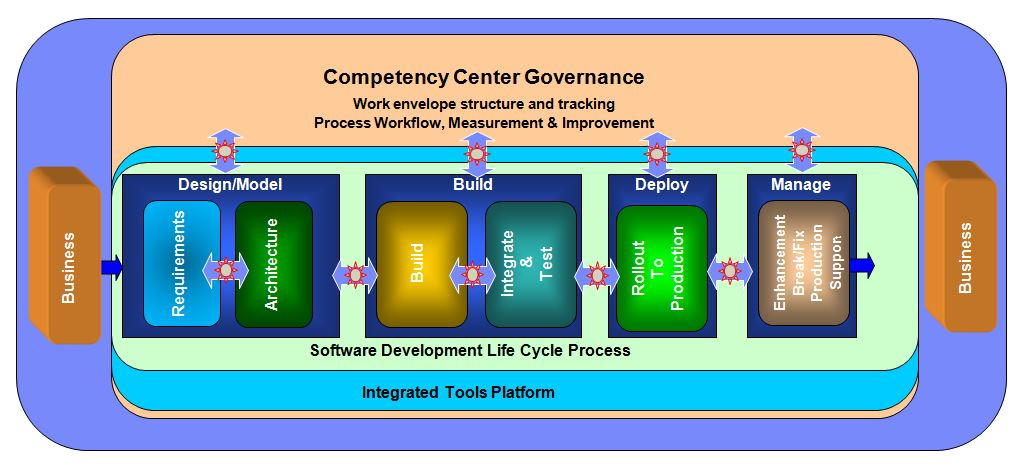
\includegraphics[bb= 0 0 750 350, scale=0.30]{figs/glocomp.jpg}
\caption{GID model with competency centers}
\label{glofig1}
\end{figure}


\subsection{Research Topic: Efficient Competency Centers}

Although the competency center model has now become central to many IT vendors and large enterprises, it has seen less interest in literature as the focus is on large scale development with a global workforce which is hard to replicate in an academic setting. However, there are several accessible research problems that can significantly improve the performance of these competency centers. We highlight five such problem areas below:

\begin{enumerate}
\item Work envelopes: Central to the concept of a competency center is the ability to partition software projects into granular work envelopes. For certain classes of development and maintenance activities -- for example in the area of packaged applications -- partitioning is natural as tasks are repeatable and the skill requirements for a class of tasks is easy to establish. Is there an equivalent construct for more complex software development?
\item Measurement: In large competency centers, performance measurement is key to ensuring efficient operation. In some ways, a competency center, due to the repeatable and comparable nature of tasks it undertakes, makes performance measurement easier. On the other hand, we find that the information reported by the practitioners of a competency center is often unreliable due to the complex structure of incentives involved. Can we take advantage of the structure of a competency center to automate the collection of information to improve its reliability? Can we create checks and balances in the information collected to validate the performance measurement?
\item Estimation: Competency centers deal with large volumes of repeatable tasks belonging to a few categories that are performed by dedicated teams. We observed that this typically reduces the variance in the estimated time required to do these tasks. The reason for the reduced variance are due to the predicability of the inputs and outputs of the tasks, standardized process and a community of developers who can share experiences and know-how. In turn, this improves our ability to predict the effort needed to complete complex software projects by a significant margin.
\item Governance: Enterprises have extended their traditional project management techniques to include competency centers. However, it is unclear whether a project-centric governance model provides the right set of checks and balances to efficiently manage the output of a distributed workforce who are working on several projects at the same time.
\item Planning and scheduling: Traditional calendar day project planning is highly inefficient in the context of a competency center since development tasks can finish either ahead of or behind schedule. Since a practitioner is not tied to a particular project in a competency center, calendar day planning requires constant replanning to ensure that we are fully utilizing available capacity. A better approach would be to use a queue based model, where the queue is managed centrally to re-prioritize the tasks in a practitioner's queue to ensure on time delivery. From a practitioner's perspective, he moves to the next task in the queue once he completes the task at hand -- if he is falling behind, the remaining tasks in his queue can be moved to other practitioners.
\end{enumerate}

\subsection{Towards distributed marketplaces}

The logical evolution of the competency center model that we discussed in the last section is to extend beyond traditional organizational boundaries -- in essence, towards a competitive distributed services marketplace. Instances of such marketplaces are already appearing - for example, services that provide coding expertise for hire such as RentACoder (www.rentacoder.com), TopCoder (www.topcoder.com) are simple examples of this model. Currently, these are seen as a novelty and thus have gained little adoption in large enterprises. In the rest of this section we will explore what it will take to make this mainstream.

 A services delivery marketplace has three key players: provider, consumer and a marketplace enabler. The consumer can use the enabler to ascertain the risks that he is taking in sourcing from a particular provider. The provider in turn gets the ability to competitively price his services based on his delivery record. The enabler provides core enabling services such as: decomposing large or complex projects so they can be executed in parallel by different providers, managing complex projects that are executed in parallel by different providers, providing service level guarantees, or performing service request validation. It is important to note that our marketplace concept is itself an abstraction for efficient service delivery. Thus, all three players can belong to the same organization, each be a different organization in the true global-marketplace sense, or any combination thereof.

 Traditional IT vendors still play a role in this conceptual services marketplace -- however, small or marginal players also have a chance to compete and grow their reputation. In this setup, there are incentives for every one to participate. For traditional IT vendors, it helps offload low margin IT services to smaller vendors with less overhead. For customers it gives an opportunity to out source small work without entering into expensive long term contracts. For the marketplace providers -- who we think will be traditional IT vendors -- it is a chance to profit from helping both providers and consumers take advantage of the marketplace by offering some guarantees.

In contrast to a marketplace for complete products, service delivery is inherently more challenging as it is difficult to capture the intent of the consumer when a service request is created. The service request should not only set forth the details of the work that is to be performed but also make provision to clearly specify risk mitigation, change management, periodic reviews, documentation requirements and exit criteria in a clear fashion to set the right expectations for both the consumer and the provider.  For example, if a code development project being worked on by a provider is not progressing as per the agreed upon schedule, a risk mitigation activity may even involve canceling the service agreement. Unless such a risk mitigation activity is clearly spelled out during the creation of the service request, it may open up avenues for misunderstanding. We anticipate that the service requests in such a marketplace will not be full fledged software projects, but of the size that can be performed in a few days or weeks by a small team of developers or even individuals. Thus, they could be elements of an agile or waterfall development process. Figure~\ref{glomarketplace} shows the conceptual instantiation of such a marketplace.

 To make this concept practical there are many challenges to be overcome some of which are common to the competency center model. The primary challenge is reducing the overhead required to partition and distribute a large software project into independent units of work that can be done by skilled developers with little or no reference to the overall project context. Open source software development is a case in point where complex software has been developed successfully through a very loosely organized set of developers. For large enterprises, this mode of development may not be suitable as it does not offer appropriate security, governance and schedule controls. Can we find a balance between the need to monitor and manage the outcome with the agility that a truly distributed services marketplace can bring to the table?

 \begin{figure}[H]
\centering
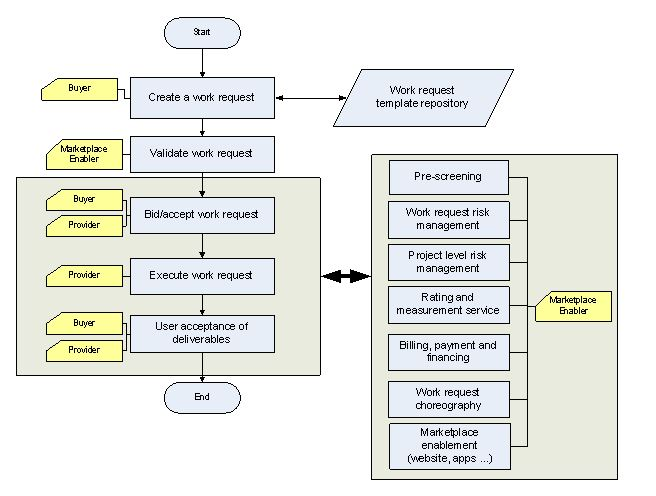
\includegraphics[bb=0 0 500 400, scale=0.5]{figs/glomarketplace.jpg}
\caption{Distributed Services Marketplace}
\label{glomarketplace}
\end{figure}

 Theoretical analysis can point to optimal regimes and controls for the efficient use of a services marketplace. Ranade and Varshney~\cite{glo-ranade} use game theoretic models to offer key insights into some key questions about crowd sourcing in general:what type of tasks should be crowd sourced under what circumstances? Their conclusion is that  the types of tasks (specialized vs generic) and the distribution of skills in the available pool of people will have a big impact on what can be effectively outsourced.

\label{sec:global}





\section{Knowledge Management}
\label{sec:km}

Software development is inherently a knowledge-intensive activity. Software
designers and developers leverage their software-development skills, along with
domain knowledge, past experiences, and the knowledge of team members, to solve
the problem at hand, such as implementing a new feature or resolving a bug.  In
small, collocated teams, knowledge management is not a big challenge---people's
expertise on different parts of a system is typically known. New team members
can use informal communication channels to identify experts and seek their help
as needed.

However, as teams increase in size or become geographically distributed,
knowledge management starts to become challenging. In large or distributed
teams, system knowledge---\eg expertise, dependencies, best practices---is
spread across multiple people, locations, and (in the case of outsourcing) even
organizations~\cite{Desouza:2006}. In such projects, a knowledge-management
system is needed to create \textit{project memories} that can serve different
needs, such as assisting new team members in identifying experts to reach out to
for specific questions, or helping existing team members determine the relevant
artifacts, and the people they might need to coordinate with, for performing a
task. Existing attempts at creating such project memories include
Hipikat~\cite{Murphy:2005} and Codebook~\cite{Begel:2010}.

%% First, it should assist new team members in understanding the project with
%% little or no face-to-face guidance and identifying experts to reach out to for
%% questions. Second, the system should help existing team members identify the
%% artifacts relevant, and the people they might need to coordinate with, for
%% performing a task. Existing attempts at creating such project memories include
%% Hipikat~\cite{Murphy:2005} and Codebook~\cite{Begel:2010}.

A service company has a large, geographically distributed employee base, with
frequent employee churn at project and organization levels. To maintain
consistent delivery quality, it is essential to manage knowledge at the project
level. Moreover, because services is a price-sensitive business, there is also
the need to be cheaper and better, by doing more with fewer or less-skilled
resources. Driven by this need to gain competitive advantage in increasingly
competitive markets, it becomes essential for companies to build
\textit{organization memories} that store the collective knowledge of past
engagements, processes, and people to increase productivity and reduce
activities that ``reinvent the wheel.'' Such a system can enable the
organization to leverage learnings and solutions from past services engagements in
the context of a new similar engagement, even when members from the past
projects are not around.

The need for organization-level knowledge bases is well established in the
management literature~\cite{davenport2000working,bollinger2001managing}. Equally
well known is the fact that creating an effective organization-wide knowledge
base is very challenging~\cite{McKinsey:1999,Harvard:1999,Ernst:1997}. There are
challenges in: (1) \textit{knowledge creation}---how to codify explicit and
tacit knowledge and motivate individuals to contribute; (2) \textit{knowledge
  retrieval}---data versus information versus knowledge; (3) \textit{knowledge
  governance}---legitimacy, relevance, and quality of contributed
knowledge. Alavi and Leidner~\cite{Alavi:2001} present a good overview of
research issues in organization knowledge management. Prior research suggests
that IT is incapable of capturing organizational knowledge
\cite{malhotra2004knowledge,mcdermott2000information}, but also postulates that
IT is the strongest enabler for organization knowledge management systems
(OKMS).

Next, we present three scenarios illustrating the need for OKMS in service
companies. Then, we discuss promising research directions based on our
experience with building systems intended to promote knowledge reuse in these
scenarios.

\subsection{Scenarios for OKMS}

In this section, we present three typical scenarios in service delivery that can
benefit from an organization knowledge management system.

\subsubsection{Troubleshooting}

One of the common forms of service engagements is application maintenance, where
the expectation from the service provider is to take over a client's custom
application and handle service requests for it.  Service requests come in the
form of trouble ``tickets'': users of the applications can raise a ticket,
logging a problem they have experienced. This is similar to defect logging in
bug repositories, such as Bugzilla, where users of an open-source software can
enter the details of a problem that they encountered.  The main difference is
that, in typical software development in open-source communities, there is no
obligation on the development team to address the defects in a timely
fashion. Likewise, even in a product setting, the development team can
prioritize which defects they are going to address first.  In service context,
the service provider is supposed to resolve the ticket in a timely manner, often
under a service-level agreement. For example, a critical bug must be resolved
within 6~hours, at risk of financial consequences for the provider.

Software development in service organizations is not pure custom
implementations---often, packaged applications, such as SAP, Oracle, and COTS
products, with client-specific customizations and external libraries are
used. The cause of a problem ticket could be in the customization done for the
client, in the way external code is used, or even a bug in the external code. If
the issue is with the configuration or the external code, it is likely that the
same (or a similar) issue has been resolved previously for another client, and
access to that information would make the people resolving the current ticket
more efficient and effective at their task.  Therefore, a knowledge base that
stores past resolved tickets across clients would be a useful organization-wide
resource.

In a way, such a knowledge base would be similar to public question-and-answer
forums we see on various software languages, tools, and open-source projects on
the web.

\subsubsection{Software Development Projects}

Another common form of service engagement is business-process transformation,
where the responsibility of the service provider is to IT-enable a business
process, such as payroll management, vendor management, or order-to-cash, for a
client. Some business processes (\eg payroll management) would be required by
all clients, whereas other processes would be common within a domain only (\eg
claim-management process in the insurance domain).  The client expectation is
that the service provider possesses adequate knowledge of the generic version of
a particular process, creates client-specific variations, and implements the
system. Typically, this requires significant domain experience.

A knowledge-management system that stores past business process implementations
can help in this scenario. The past solutions need to be organized by domain for
easy retrieval of relevant information. Appropriate documentation that explains
the standard and customized portions of past solutions needs to be available,
along with the solution code. While designing a new business-process solution,
the team can search the repository to learn about variations of the process to
be implemented and, if the client requirements are similar to a past solution,
even reuse the solution in totality or parts. This can reduce the cost and
let the service provider staff the team with people with less domain experience.

Code reuse, at different levels of granularity---lines-of-code level, API level,
and even complete solutions---has been an area of interest in the
software-engineering community~\cite{Reiss:2009,Holmes:2013}. Much of this work
could be applied in the setting of a service company too. In services engagements, because the code is being developed for a particular client, who owns the code IP might become an issue. If the code ownership is solely held by the client, making the solution code available as part of a shared repository would not be possible. Services organizations often face this challenge of convincing the clients of sharing artifacts created as part of these individual engagements into cross-account repositories maintained by the service providers. Experience reports, user studies that report on effort reduction and/or quality improvement from code reuse can enable service organizations to quantitatively convince the clients of benefit they are likely to receive because of actual software artifact sharing and reuse.  

\subsubsection{Service Improvement}

When a client outsources application maintenance to a vendor, one of the key
expectations is that the vendor would bring down their total cost of ownership
over time. This requires the vendor to seek out proactively areas for
improvement in the client application portfolio. One way to do this is via
benchmarking the performance of the client applications against similar
applications in other client landscapes. To illustrate, suppose that a service
company maintains the payroll applications for 10~clients. For nine of the
clients, the monthly ticket volumes range between 5 and 10 tickets, whereas, for
the remaining client (say client~A), the ticket volume ranges from 20 to
50. This indicates that, for client~A, it may be worthwhile to investigate
reasons for high ticket volumes and determine whether preventive actions can be
taken. Moreover, if a similar problem was seen in the past in another client's
payroll system, information about the actions taken for that client could help
the team resolve the problem for client~A.

Many organizations (\eg CAST, Software Engineering Institute) collect
quantitative and qualitative benchmark information for software projects and
business applications based on languages used, number of users, etc.  For a
service company, which does software implementations for multiple clients, an
organization-wide knowledge base that (1) captures key operational metrics per
application (or by problem area) and the past improvement actions taken for each
client, and (2) permits comparisons between clients with similar applications
and problems encountered, would improve upon what is publicly available and be
more useful.

%% There are a number of organizations that gather and report quantitative
%% benchmark information (qualitiative as well as productivity) for software
%% projects and business applications depending on language used to code, number of
%% users etc. CAST, Software Engineering Institute are some examples of such
%% organizations. However, considering services organizations are doing multiple
%% software implementations for multiple clients, an organization-wide knowledge
%% base that (1) captures key operational metrics per application (or at a more
%% granular level, such as by problem area) per client and the past improvement
%% actions taken, and (2) allows comparisons between clients with similar
%% applications and problems encountered, would help augment what is publicly
%% available and be more useful.

\begin{figure}[t]
	\center
	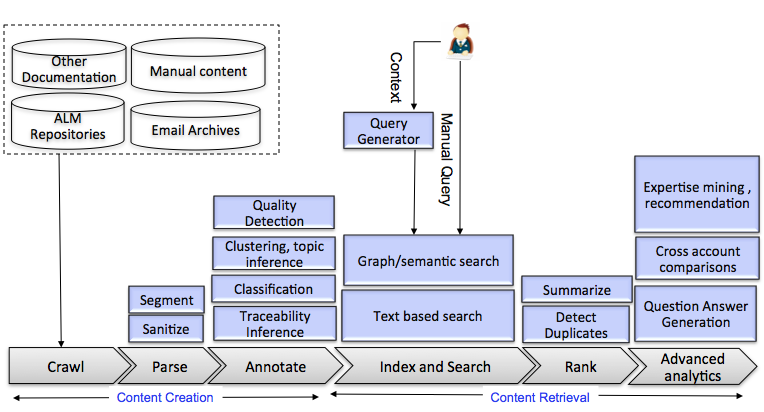
\includegraphics[width=\columnwidth]{figs/km.png}
        \vspace*{-18pt}
	\caption{Activities involved and tasks performed in building and using
          an OKMS system for a service company.}
        \vspace*{-10pt}
	\label{fig-km}
\end{figure}

\subsection{Research Topics}

Based on such OKMS needs in IBM's service-delivery organization, there have been
efforts toward implementing systems to address the needs. These include a system
for promoting solution reuse in software development engagements centered around
business-process transformation~\cite{Goodwin:2012b}, and a system for sharing
information about problem tickets across client
engagements~\cite{Majumdar:2011}.

We next discuss some core problems that need to be addressed in creating an OKMS
in service organizations. At the simplest level, an OKMS is a database where
content can be stored and retrieved from. However, what content should be
stored, how easily can the requisite content be collected, and the ease with which relevant
content can be retrieved determines the usefulness of an OKMS.
Figure~\ref{fig-km} presents several activities (shown as block arrows) that
need to be performed in creating and using an OKMS; for each activity, the
figure displays relevant topics (shown in the boxes) that would benefit from
further research. The activities are broadly classified into two categories:
knowledge creation and knowledge retrieval.


\subsubsection{Knowledge Creation}

What constitutes useful knowledge in a service company? How can such knowledge
be collected and organized? These are some of the questions that need to be
addressed in knowledge creation. Specifically, we discuss three aspects of
knowledge creation: \textit{crawling}, to collect content from diverse
sources; \textit{parsing}, to translate the content in various formats into a
standard format; and \textit{annotating}, to extract metadata from the content
that can help organize it.

\vskip -5pt
\paragraph*{Crawling} The first activity in building an OKMS is
identifying the data that should be stored in the repository and how to obtain
the data. In general, this activity includes a combination of manually provided
data and automatically crawled data, each of which can have its own peculiar
challenges.

For manual data collection, an organization can require its employees to
contribute learnings and software artifacts to the OKMS. For instance, this
could be done via FAQs, where employees outline solutions to common problem
tickets they have resolved; or, it could be done via postmortem reports, usage
stories, and experience reports~\cite{desouza:2005} created by project members
after the resolution of a key project issue. If a client solution involves
software development, employees can be asked to identify reusable software
components and contribute them, after generalization, to the OKMS.

Manual content creation puts extra burden on the employees, beyond their normal
delivery-related responsibilities. Thus, an interesting problem is how to
motivate employees to contribute high-quality content to the
OKMS~\cite{hendriks1999share}. Incentive mechanisms could include ``badges'' as
is done in open-source forums, such as stack exchange to encourage question and
answer contributions. In a service company, would reputation-building incentives
be sufficient or would monetary or career-growth incentives be
necessary~\cite{bartol2002encouraging}?

%% An organization has the option of mandating that each of it's employees
%% contributes their learnings to the OKMS system. Some examples of manual
%% knowledge creations are: (1) frequently asked question, where employee outlines
%% the typical solutions to some common problem tickets they have resolved (2)
%% postmortem reports, usage stories, experience reports\cite{desouza:2005}, that
%% project members can create after they solve a key issue in the project. To
%% enable solution reuse, services organizations often invest in creating software
%% product families
%% \cite{clements2002software}. However, here it's pre-anticipated what could be
%% some solutions that could be of interest to multiple clients in a particular
%% domain such as healthcare and then those solutions are created with appropriate
%% points for variability built in, so solution can be customized for any client
%% intending to use it.  Once a project is completed, employees are also encouraged
%% to identify reusable components in software they created and share them in the
%% knowledge base. This approach of manual content creation adds extra burden on
%% the employees. An open research challenge is to motivate employees to contribute
%% high quality content in the knowledge base \cite{hendriks1999share}. Open source
%% forums such as stack exchange have experimented with elaborate incentive
%% mechanisms in forms of badges to ensure questions and answer contributions on
%% their forums \cite{vasilescu2014social}. In services organizations are
%% reputation building incentives enough or incentives should translate to monetory
%% benefits and/or career progression /cite{bartol2002encouraging}?

In addition, or as an alternative, to manual content creation, content can be
collected through automated crawling of the artifacts produced in a project. For
example, complete traceability from requirements through code to test cases,
along with relevant content, can be extracted from Application Lifecycle
Management tools. Similarly, information about problem tickets and their
resolutions can be extracted from ticket-management systems.  Account teams
periodically report important metrics, such as ticket volumes, code changes, and
service-improvement actions taken, on the client applications being maintained;
these reports could be automatically pushed into the OKMS. The main challenge
here is extraction of this data from the diversity of tools and technologies used to create software
artifacts and related information across projects.

%% Another approach for content creation is to auto-harvest artifacts produced in
%% the SDLC lifecycle and put these in the knowledge management system. Complete
%% traceability from requirement through code to test cases, along with their
%% content is extractable from Application Lifecycle Management tools and this can
%% act as solution packs to put in the repository. Similarly for ticket resolution,
%% information about problem ticket and it's resolution is extractable from ticket
%% management systems. Account teams periodically report on various important
%% metrics on the applications being maintained in the client landscape such as
%% ticket volumes, code changes, service improvement actions taken. These reports
%% can be auto pushed into the knowledge repository. The main challenge here is
%% handling the diversity of tools and technologies used to create SDLC data across
%% projects.

\vskip -5pt
\paragraph*{Parsing} After data has been pulled from various
sources, the next activity involves parsing different document formats and
templates into a standardized format that can be pushed into the knowledge
repository. The diversity of formats, some of which may be proprietary, makes
automated content parsing a challenging problem and a fruitful research
direction. For instance, a possible approach could be based on writing
model-to-model transforms~\cite{debdoot:2010:scc}.

Another issue is that the traceability information necessary for understanding
the context of how and why an artifact was produced might be missing---for
instance, traceability between code commits and bug reports is necessary to support knowledge reuse for troubleshooting. Similarly, traceability between requirements and application code is desired to enable reuse of business process software implementations across projects. The gaps in traceability  occur
primarily due to lack of integration between the tools used to create the
artifacts. In such cases, automated analyses must be developed for inferring the
traceability; this is an active area of research~\cite{spanoudakis2005software},
with different types of approaches, such as those based on information
retrieval, traceability rules, special integrators, and inference axioms, being
developed.

%% \paragraph*{Parsing} Once all the requisite data has been pulled from various
%% sources, the main challenge is parsing of the data from various document formats
%% and templates into a standardized format that can be pushed into the knowledge
%% repository. Many of the crawled data is in form of documents in proprietery
%% formats such as Microsoft word, power point slides, visio diagrams, excel
%% sheets. How to automate content extraction from client specific work products
%% into the standard format used by knowledge repository is again a direction for
%% research. One approach is to write model to model transforms where a project
%% admin can specify the mapping \cite{debdoot:2010:scc}. Another challenge is that
%% requisite traceability information that is required to understand complete
%% context of how and why an artifact was produced, might be missing. This is
%% because tools being used to create different SDLC artifacts have not been
%% integrated. There is need to auto infer traceability between artifacts For
%% example, if making a code commit, the developer puts in a comment like "Fixed
%% Bug \#145", then with high confidence the change is to fix "Bug \#145" and
%% traceability edge between code file and bug report should be auto-created.
%% . Tracability inference is an active area of
%% research \cite{spanoudakis2005software}. Some proposed approaches use
%% information retrieval (IR) techniques, others use traceability rules, special
%% integrators, and inference axioms.

In service delivery, the OKMS is populated with data collected at client
engagements and can include client-confidential and sensitive information (\eg a
problem ticket might contain the contact information of the user). Thus, a
critical requirement for the OKMS, which would benefit from automation, is
cleansing or anonymization of all sensitive and client-confidential information.

%% The content in a OKMS database comes from various clients:. There are strict
%% privacy constraints around what data is client confidential and hence cannot be
%% shared. Within a single artifact itself, there might be small portions of
%% content that are client confidential. E.g. a problem ticket might content the
%% contact information of the user who encountered the information. How to remove
%% client confidential data from artifacts put in the repository, how to anonimize
%% the content so as to not disclose client identity and how to ensure that only
%% authorized users and roles have access.

\vskip -5pt
\paragraph*{Annotating}
The content in the OKMS must be organized for easy retrieval. The general
practice to do this is to classify OKMS content against predefined
taxonomies. For example, a simple taxonomy is the artifact type: requirement,
code, problem ticket, etc. More generally, a taxonomy ought to include
information about industry type and process area~\cite{apqc,bph}, technologies
used, etc. Organizations spend effort in building and maintaining these
taxonomies; automated tool support to assist with this would be useful. For
instance, clustering~\cite{Berkhin06} and topic-modeling
techniques~\cite{Blei:2012} could be leveraged to group similar content and
infer topics from them.

Manual classification of data can be tedious and prone to human errors. To
reduce this effort, automation via pattern matching and machine-learning-based
classification approaches~\cite{bishop2006pattern} could be used.  The
effectiveness of these techniques depends on the availability of positive and
negative samples to train a learning model. Often, due to unavailability of
training data and/or lack of differentiating features, usual learning techniques
such as na\"{\i}ve bayes, support vector machines, and decision
trees, do not attain sufficient precision and recall. Thus, there is a
need to customize more advanced learning approaches (\eg
ensemble techniques~\cite{Dietterich:2000}) or develop new techniques that are more effective
on the typical data available in service delivery.

%% One taxonomy is obviously the object type i.e. requirement, code,
%% problem ticket (further segmented into problem description, resolution). Another
%% taxonomy captures the domain the artifact was produced in i.e. industry type and
%% process area e.g. \cite{apqc,bph}. Another taxonomy is the technology
%% used. Organizations spend effort building and maintaining these taxonomies. For
%% every data that is put into the knowledge base, the content needs to be manually
%% categorized against these pre-defined taxonomies. Pattern matching and machine
%% learning based classification approaches /cite{bishop2006pattern} can be used to
%% auto-categorize content to these pre-defined taxonomies. These techniques rely
%% on the availability of equal proportion of positive and negative samples to
%% train a learning model. However, due to unavailability of training data and/or
%% lack of differentiating features, usual learning techniques such as naive bayes,
%% support vector machines, decision trees, might end up not giving desired
%% efficacy (measured as precision and recall). There is need to customize more
%% advanced learning approaches such as adaptive learning, ensemble techniques or
%% develop new techniques that work well with SDLC data. Another interesting area
%% for research is to explore how to help grow the taxonomy over time based on
%% content coming in the knowledge base. Techniques such as
%% clustering \cite{Berkhin06}, topic modeling \cite{Blei:2012} help group together
%% similar looking content and infer topics out of them.


The data in an OKMS can quickly grow very large. For example, in just a year, a
problem ticket repository we setup in IBM grew to contain 750,000 tickets;
similarly, our business process solution repository~\cite{Goodwin:2012b}
contains approximately 16,000 solutions. Given this scale, ensuring high quality
of the data (\eg filtering out non-reusable content) is challenging but
essential. Different approaches could be followed for ensuring data quality,
such as human vetting of incoming OKMS content or based on human feedback on
usefulness of retrieved content. An interesting research direction would be to
explore automatic quality scoring of artifacts, taking into consideration
technical and non-technical artifact content, reputation of artifact authors,
etc. For example, such approaches have been investigated
in~\cite{Majumdar:2011}.

%% Once an OKMS system is implemented in an organization, irrespective of the
%% approach to collect content i.e. manual, automated harvesting or hybrid, the
%% repository starts filling up fast. Over a period of one year, the problem ticket
%% repository we setup within IBM collected 750K tickets. Similarly, the business
%% process solution repository has 16000 solutions. However, not all content being
%% put in the repository is high quality and reusable. Hence, it is becomes
%% imperative to be able to filter out useless content. One way to achieve this is
%% by making a human vet every content being pushed in the repository and only
%% content that is deemed high quality is published. Another approach is to ask
%% people who are retrieving and potentially using the content, give feedback on
%% whether they found content useful or not. The third approach that makes for an
%% interesting research direction is to explore how a an automatic quality score
%% can be assiged to each artifact based on content in the artifact, prior
%% reputation of people who authored the content, whether the project was a success
%% or not and so on. In our problem ticket repository, we experimented with
%% calculating a quality score per ticket based on technical versus non-technical
%% content present in the ticket \cite{Majumdar:2011}.


%% \paragraph*{Summary} To summarize, content creation in OKMS provides multiple
%% oppurtunities where research can contribute. These include: what and how to
%% extract content from SDLC repositories and proprietry document formats, how to
%% infer traceability between different artifacts, how to classify and categorize
%% content, how to maintain privacy, estimate quality and motivate employees to
%% contribute high quality content.


\vspace{-5pt}
\subsubsection{Knowledge Retrieval}

Challenges in knowledge retrieval are related to the search capabilities offered
by the OKMS and the effort required from users in determining the usefulness of
the recommended data. We discuss the following aspects of knowledge retrieval:
indexing and searching, search result organization, and advanced analytics.

\vskip -5pt
\paragraph*{Indexing and Searching} The simplest approach for searching
is \textit{keyword-based search}, in which users specify the words they are
looking for and the system returns all artifacts that contain the specified
words. More sophisticated systems use \textit{faceted search}, where the user
can navigate a hierarchical structure (\eg a taxonomy) and select values from
predefined categories.  Despite the availability of many search technologies,
studies such as \cite{idc2}) have shown that retrieval of relevant information
from organizational repositories remains challenging, with users being
successful in less than 50\% of their attempts in searching for information.

Language-based information-retrieval techniques~\cite{manning2008introduction},
on which many knowledge systems are based, may be inadequate in dealing with the
types of repositories we are talking about---that contain not just a collection
of artifacts, but a network of linked artifacts.  Graph databases for storage
and semantic search techniques~\cite{Guha:2003} or extending keyword search for
graphs~\cite{kacholia2005bidirectional} may be more promising in this scenario,
and are worthy of research investigation.

%% \paragraph*{Index and Search} Indexing is how the knowledge repository stores
%% data internally. Search features then work on this index.  Typical ways to
%% retrieve content from a knowledge base are: (1) keyword based search where user
%% specifies a couple of words (s)he is looking for and all artifacts in the
%% repository that contain the words from user query are returned, (2) faceted (or
%% navigational) search where user is shown a hierarchy structure (taxonomy) and
%% can browse information by choosing one or more values from each of the
%% pre-defined categories. Various language based information retrieval
%% models \cite{manning2008introduction} such as vector space models, probablistic
%% models, latent semantic index exist that can be used here. But inspite of easy
%% to use search technologies being available, prior studies report that knowledge
%% retrieval from organization wide repositories remains a challenge. As
%% per \cite{idc,idc2}, while employees spend 15\% to 35\% of their time searching
%% for information in an enterprise, they are successful less than 50\% of the time
%% in finding what they are looking for. Most existing OKMS systems use language
%% based IR models to store and retrieve knowledge. However, as we saw in content
%% creation section, the repository is not just a collection of artifacts but a
%% network of linked artifacts. Use of graph databases for data storage and
%% retrieval techniques such as semantic search techniques \cite{Guha:2003} or
%% optimizing keyword search for graphs \cite{kacholia2005bidirectional}, are worth
%% exploring.

An important factor in performing accurate search is the expressiveness of query
construction. Simple keyword queries, consisting of a set of words, may not be
discriminative enough to return accurate results. A few approaches have been
developed to address this problem, for example, by giving more weights to words
that appear in the title of a problem ticket than words that appear in the
ticket description~\cite{Sinha:2012}, and using separate queries for different
types of information, such as description, application information, and stack
trace, in a problem ticket~\cite{Ashok:2009}.

Another question pertains to assigning weights to clauses in the query while
ranking the search results~\cite{Debdoot:2011:bpm}. Moreover, the idea
of \textit{contextual search}~\cite{wen2004probabilistic,kraft2005q}, which
attempts to capture the user's information needs better by augmenting the query
with contextual information extracted from search context, has shown promising
results. Further research along these directions---in the context of the
knowledge needs in service delivery---investigating different ways of creating
contexts, using contexts in constructing queries, and assigning weights to query
clauses would be interesting.

%% Non-availability of content or poorly organized content can be one reason for
%% this. Another reason could be the inadequacy of the query itself that are used
%% to retrive the content. Suppose a user is trying to find problem tickets that
%% resolved similar issues to what (s)he has been assigned. (S)he would pick up a
%% couple of words from the ticket that describe the problem and use it to query
%% the knowledge base. However, these words might not be discriminative enough and
%% user might end up getting too many or too little search hits. Another approach
%% could be to use complete content in the ticket and use it as query. However in
%% this case, the search engine might end up returning irrelevant results as equal
%% weightage was given to all words in the problem ticket. \cite{Sinha:2012} tries
%% to address this issue by giving more weightage to those words in the query that
%% belong to ticket title. \cite{Ashok:2009} parses out different datatypes from a
%% problem ticket such as description, application information, stack trace and
%% using a different query/search mechanism for each. E.g. instead of just
%% specifying "null pointer exception", the query generated from a problem ticket
%% could be---description: contains following bag of words \{null, pointer,
%% exception\}, process: is equal to "order to cash", stack trace: contains
%% foo.*bar. The results obtained from such a query are likely to be more precise
%% than what a keyword search would yield. A challenge with this approach is how to
%% compose the various clauses in the query---are they "anded" or "ored" or a
%% combination. Another challenge is how much weightage to give to each clause when
%% ranking the search results \cite{Debdoot:2011:bpm}. Moreover, recently
%% contextual search \cite{wen2004probabilistic,kraft2005q} has been gaining
%% momentum. Contextual search tries to better capture a user's information need by
%% augmenting the query with contextual information extracted from search
%% context. It would be an interesting direction for future research to see for
%% each of the knowledge needs in services organizations, what can make up the
%% context, how to use this context to create the query and how to weigh different
%% clauses in the query.

\vskip -5pt
\paragraph*{Search Result Organization}
Although more powerful querying capabilities can help improve the accuracy of
search results, a search-based system would in general return multiple
results. The next question then is: how much effort does it take for the user to
sift through the results to find relevant information? Simple approaches such as
highlighting matching keywords will not work for complex queries; more
sophisticated techniques that help the user easily comprehend the relevance of
the results are needed. One such approach is \textit{summarization}, which has
been used in text-processing domains to end users get a quick overview of
information; summarization has also been applied to bug
reports~\cite{Mani:2012,Rastkar:2010}. Extending this notion to other types of
artifacts, such as code, requirements, and solution designs, is an open topic
for research.

Another type of analysis that can improve the search results is detection and
grouping of duplicates or near-duplicates. By grouping together such artifacts
and highlighting the variances in seemingly similar artifacts, the system can
reduce information overload on the user.  Detection of duplicate bug reports has
been widely researched
(\eg \cite{wang2008approach,sun2010discriminative}). Developing such analyses
for other types of artifacts, from a services OKMS perspective, would be useful.

Typically, an OKMS would display the search results as a ranked list, with
10--20 items per page. The ranking can be based on relevance of artifacts,
quality of artifacts, past user ratings given to artifacts, etc. Prior research
have explored other novel ways to visualize search results
(\eg \cite{Nowell:1996,Shneiderman:2000}).  Another potential direction for
research is the investigation of effective non-list visualizations of OKMS
artifacts.

%% What kinds of non-list visualization
%% would be effective in organization knowledge management system that are
%% predominantly composed of SDLC artifacts is another direction for research.

%% \paragraph*{Search Result Organization}
%% Any search based system would return multiple results. For the user it becomes a
%% chore in itself to go over each of the search results and identify if it is
%% relevant or not. Techniques that can help the user easily comprehend the
%% relevance of the returned results are much needed. Text based search engines
%% highlight the matching words between query and content of the artifact
%% returned. However, when the query becomes complex (as above), keyword
%% highlighting is not of much help. In text processing domain, summarization is
%% one approach that is used to help end users get a quick idea of what the content
%% is about. In \cite{Mani:2012,Rastkar:2010} authors present different techniques
%% to summarize bug reports. Research can help in developing summarization
%% techniques that work for other SDLC artifact such as code, requirements,
%% solution design documents and so on. Further, out of the search results returned
%% many artifacts could be duplicates or near duplicates of each other. In order to
%% reduce information overload for end user, the OKMS system should be able to
%% group together duplicates and near duplicates and be able to highlight the
%% variances in seemingly similar artifacts returned in the search
%% results. Duplicate bug report
%% detection \cite{wang2008approach,sun2010discriminative} has been a widely
%% researched topic. Similarly for each of the artifact of interest from a services
%% OKMS perspective, a customized duplicate detection approach might be needed.

\vskip -5pt
\paragraph*{Advanced Analytics}
Most knowledge-management systems today stop at providing search
capabilities. Given the magnitude of data that can be collected in OKMS, there
is the opportunity of implementing advanced analytics that go beyond by
supporting decision making. Consider the scenario of troubleshooting where, to
resolve a ticket, the user searches through past resolved tickets to find
similar tickets.  Based on the past tickets and the current context, the user
has to formulate potential hypotheses about the root cause, decide which
hypotheses are applicable, and then investigate the solutions. The OKMS would be
much more useful if it could automatically generate potential hypotheses about
root causes and solutions for the user to investigate.

Service requests or tickets contain a lot of information in unstructured text format. Textual analytics applied on this data can help provide useful insights. For example, clustering on service tickets text could help identify problem areas that are causing higher maintanence grief and hence are good candidates for doing preventive work. This approach is discussed in \cite{mani2014}. Analysis of groups of similar problems and resolutions can be used to auto extract out frequently asked question and answers from service requests. In \cite{henss12} authors have presented a text mining and natural language processing based approach to extract FAQs from questions being asked on mailing lists of open source projects.

The effectiveness of knowledge retrieval in the context of service delivery
depends to a large extent on the user's ability to identify projects similar to
the project under consideration. What makes two projects similar? Is it the
technologies being used, the project size, similarity of applications, or a
combination of these and other factors? Investigation of this question and
development of automated techniques for identifying similar projects is needed.

%% \paragraph*{Advanced Analytics}
%% OKMS today stops at providing search capabilities. Given a user query, the
%% system returns back matching artifacts but makes no attempt at making any
%% deductions. Consider the scenario of troubleshooting. A user is searching
%% through the past resolved ticket repository to see if similar issues were
%% resolved. There are multiple reasons why the issues could have arisen. Based on
%% past tickets, the user needs to come up with potential hypothesis of why the
%% issue could be arising and based on conditions (s)he is seeing in the current
%% landscape decide what hypothesis is applicable and then pick the appropriate
%% solution. From such a user's perspective the OKMS system would be more effective
%% if it were able to auto-generate these potential root causes and solutions
%% hypothesis. Consider the service improvement use case, the accout team needs
%% support from OKMS to identify similar projects, then compare the problems seen
%% in the current project with different kind of issues arising in similar
%% projects, then judge whether current team is doing better or worse and then
%% decide to take some action. What kind of capabilities are needed in OKMS system
%% to be useful in above scenarios is another area for research.

%% Much of the knowledge retrieval first requires that user is able to identify
%% similar projects in the organization and then dig deeper into them for learning
%% or comparison with situation at hand. What makes two projects similar? Is it
%% technologies being used or project size or similarity in applications or a
%% combination? Hence, analysis to identify similar projects, compare a project
%% against multiple other projects and auto-summarize similarities and differences
%% is needed.

In general, there are two aspects of organization knowledge management:
codification and personalization~\cite{hansen2000s}. Our discussion of OKMS has
so far focused on the codification aspect, where knowledge is carefully captured
and stored in a knowledge base for use by anyone in the company. The
personalization aspect ties knowledge to specific people; the main purpose of
knowledge management here is to help the user find and connect with people who
have the requisite knowledge, not store the knowledge. This strategy is
especially appropriate in cases where knowledge cannot be easily codified, such
as the knowledge for handling situations that require complex decision
making. Expertise browsing, recommendation, and mining have been explored in
various contexts (\eg \cite{Balog:2006, Mockus:2002}). Extending
these ideas to the context of service delivery, where the OKMS contains data
from multiple projects in different contexts, is an area where further research
can help.

%% There are two techniques for organization knowledge management, codification or
%% personalization \cite{hansen2000s}.  Till now what we have discussed is what is
%% called codification. Here knowledge is carefully captured and stored in the
%% database, where it can be accessed and used by anyone in the company. This
%% strategy allows many people to search for and retrieve knowledge without having
%% to contact the person who originally developed it. This opens up the possibility
%% of achieving required scale in knowledge reuse in services
%% organizations. Another strategy for knowledge management is
%% personalization. Here knowledge is tied to person who developed is and is shared
%% mainly through direct person-to-person contacts. The chief purpose of knowledge
%% management system here is to help people find and connect to other people who
%% have requisite knowledge, not to store it. This strategy works well when
%% knowledge cannot be codified especially knowledge required to handle situations
%% that require complex decision making. Expertise browser \cite{Mockus:2002},
%% expertise recommender \cite{McDonald:2000} have attempted to identify experts on
%% various topics within a project. \cite{Balog:2006} has explored expertise mining
%% and recommendation in predominantly document based OKMS systems. What
%% information to use to mine expertise when repository contains SDLC data from
%% multiple projects, how to match your current context and job profile to suggest
%% people you should have in your network is another scenario where research can
%% help.

%% \paragraph*{Summary} To summarize, content retrieval in OKMS system provides
%% open research problems in query generation and use of context to augment
%% queries, search result summarization, duplicate detection, use of semantic
%% search to improve search relevance. Further the retrieval capabilities need to
%% move beyond just search to provide capabilities such as question-answer
%% generation, cross-account comparison/benchmarking and expertise recommendation.




%\section{Troubleshooting}

One of the common forms of service engagements is application maintenance, where the expectation from the service provider is to take over a client's custom application and handle service requests for it.  Service requests come in the form of trouble ``tickets'': users of the applications can raise a ``ticket'', logging a problem they have been experiencing. This is similar to bug repositories such as Bugzilla, in which users of an open-source software can enter the details of a problem that they experience.  The main difference is that in typical software development in open-source communities, there is no obligation on the part of software maintainers to address the defects in a timely fashion. Likewise, even in a product setting, the development team can prioritize which defects they are going to address first.  In service context, the service provider is supposed to resolve the ticket in a timely manner, often under a service-level agreement. For example, a critical bug must be resolved within 6 hours, at risk of financial consequences for the provider. 

Clearly, the efficiency which the service provider can resolve these tickets is a differentiating factor. For this reason, troubleshooting is a important research area for software services.

Ticket resolution takes place in stages. At the front, customer facing level is what is called L1 support, which simple acknowledges the issue to the customer and assigns it to an internal queue. In simple cases, such as request for information, L1 support can provide ``help desk'' features. L2 support comes in when the ticket requires technical expertise to answer, but usually resolving the ticket entails no more than advising the customer of the right configuration, or a workaround, etc. Finally L3 support handles real defect, and resolving them typically involves fixing the code.

(We can use a picture here.)

L1 and L2 support can benefit from the techniques that we reviewed in the section on knowledge management.

Here we describe some of the challenges in L3 ticket resolution.

In the purest form, the troubleshooting problem (a.k.a. debugging) is this: given the symptom of a defect, such as an incorrect output, how do you efficiently determine the fix to the code ?  We distinguish code level problems from architectural problems. Resolving architecture problems require a major transformation effort, outside the scope of troubleshooting.

While troubleshooting is par for the course in software industry as a whole, things are a bit different for the services part. First, efficiency in troubleshooting is strongly linked to the bottom-line of the provider, and the companies compete on the basis of this efficiency. Second, service providers may not have long-term ownership of the application code. They often have to ramp up quickly, often without access to the developers who originally wrote the code. For these reasons, as important as tools for faster troubleshooting are for product developers, they are perhaps even more crucial for services companies.


\section{Risk identification and management}


Software risk management is a well established discipline~\cite{risk1,risk2} that has generated continued academic interest as the complexity and nature of the software projects have evolved over time. Traditional risk management techniques have been focused on identifying and codifying best practices that prevent or reduce the failure rate~\cite{risk3,risk4,risk5,risk6,risk7}. Large IT organizations have assimilated many of these findings in their risk management practice.  However, adopting these best practices does not guarantee that risk is eliminated or even reduced to an acceptable level -- new software development models driven by globalization, competition and an ever changing software landscape throw up new patterns of trouble.

In recent literature, the trend towards a systems approach to risk management, where in statistical techniques are used to classify and mine the project metrics data, with a view to pro-actively learn the new trends is gaining acceptance~\cite{risk8,risk9,risk10}.  These methods actively use the metrics collected during traditional risk management reviews and then employ techniques borrowed from statistical learning theory to derive models that describe the relationship between the collected metrics and eventual project outcomes. Thus, certain patterns of values in project metrics can act as alerts, which can be then used to initiate further reviews to see whether the alert was justified. It is important to note that these techniques in most cases cannot identify why a project may be troubled i.e., they can only serve as a starting point for further investigation.  Another significant short coming of these models is their inability to implicitly account for outliers and missing data -- for example, a project in good health will not typically have as thorough a review as a project in trouble9. Unless the data that is used to train the model is carefully validated to account for these characteristic patterns, there is a good chance that the model will not be very accurate. This problem is particularly prevalent in large IT delivery organizations which typically exhibit a large variance in both the quality of the metrics collected and reporting patterns.

Functionality risk is defined as the risk that the completed system will not meet its user's needs~\cite{risk11}.  It is the risk that churn in business requirements and scope combined with ineffective communication mechanisms leads to the development of working software that is essentially useless to the end user~\cite{risk12}. In a recent article~\cite{risk13}, it has been argued that functionality risk has become an increasingly important factor due to the challenges  that globalization has created. Through empirical analysis, they identify that development methodology fit, customer involvement, and use of formal project management practices as the top three functionality risk factors. In complex IT engagements we find that reducing or eliminating functionality risk, which in turn leads to high customer satisfaction, may result in an unacceptable increase in other risk factors such as financial risk for the provider. Thus, in our approach we opt to look for trouble patterns across a broad spectrum of risk indicators and surface problems which then allow risk managers to make informed decisions.

Quantitative analysis of IT investment decisions using options analysis, to mitigate financial risk, is an active area of research~\cite{14,15,16}. Options analysis can be used to assess the value of prototyping work and early adoption initiatives related to new IT platforms – options provide a way to evaluate the value of IT projects which give the right to adopt the resulting technology without having the obligation to do so. Fichman~\cite{risk14} shows how options analysis can be used to predict IT platform initiation and adoption, value IT platform options and manage IT platform implementation. Chen and Sheng~\cite{risk15} discuss how to do real options analysis while accounting for estimation errors. However, the ability to use the results of the analysis in a dispassionate manner to start and cull IT projects is still a contentious topic~\cite{risk17}. As Keil et al.~\cite{risk18} observe, there is a strong bias in many organizations to continue with IT projects even though financial analysis indicates otherwise. In our view, the lack of widespread adoption for options analysis can be traced back to a fundamental issue that effects all methods for analyzing financial risk – the inability to accurately estimate with any degree of certainty the net present value (NPV) of a complex in-flight IT project. In this paper,  we evaluate financial risk by analyzing how projects that exhibited similar trends in project metrics performed in the past – thus, the analysis has no dependence on a particular methodology for evaluating NPV.

Evaluating IT project portfolios with a view to making strategic decisions that help the portfolio grow in accordance with business needs helps target limited budgets on relevant projects. Armour~\cite{risk18} argues that a company’s IT project portfolio should be treated like any other investment portfolio to understand whether the reward justifies the estimated risk. Given the uncertainty surrounding the estimation of risk, Lin~\cite{risk20} suggests that fuzzy logic may be used to make IT portfolio decisions. Holland and Fathi~\cite{risk25} suggest that uncertainty can be reduced through portfolio diversification and spreading the risk of incorrect risk management decisions across a wide pool of projects. Our approach to surfacing trouble indicators provides tools for a company to make strategic decisions about its IT project portfolio.

Erickson and Evaristo~\cite{risk22} provide an account of how risk factors associated with IT projects are magnified or multiplied when dealing with distributed project teams.  They provide a conceptual list of a variety of factors ranging from culture to distance and discuss how an increase in distributedness along these dimensions affects project risk.  Ramasubbu and Balan~\cite{risk23} present an empirical study which quantifies the loss in quality and increase in schedule risk that one would expect in global software projects. They suggest that good software process controls may mitigate these losses to some degree. Beise~\cite{risk24} suggests that good project management practices when properly applied may help to mitigate some of the problems caused by virtual teams. Our analysis suggests that even under the best possible control structure the losses due to distributed development are unavoidable -- the ability to recognize the symptoms and act quickly will decide which  companies will succeed in leveraging the promise of globalization.

It is well known that decision-makers, including those in the risk management community, routinely use flawed heuristics in decision-making, which are subject to systematic biases~\cite{risk27}. Heemstra~\cite{risk24} analyzes how filters and biases of personnel involved in judging a project may prevent an accurate risk assessment. He suggests a team based decision making approach to avoid being heavily influenced by particular individuals. Host and Lindholm~\cite{risk25}  do an empirical analysis of how a set of identified project risks are weighted by different individuals. They find a wide variance in the perceived importance attached to individual risk factors -- however, they could not explain this variance on the basis of the particular role played by the person in the project. Maytorena~\cite{risk26} provides an interesting study on the effect of experience on the ability of project managers to recognize certain risk factors. It shows that experience does not have a significant impact on the ability to detect risk as do other factors like risk management training, ability to quickly grasp information and the level of education. In practice, we find that packaging the statistical information and trouble patterns in an easily understandable and actionable fashion to the risk managers may be as important as the information itself.

\subsection{Risk prediction}
 In any complex software development project, a number of risk assessment related activities are conducted prior to project inception with an objective of determining the risk entailed in delivery. The number and depth of these reviews is determined by a variety of factors, such as: the size of the project, the novelty of the proposed solution, and the industry sector to which the client belongs. These reviews may cross multiple delivery organizations within and beyond the purview of the primary service provider who is responsible for the delivery of the integrated software solution. Even for a large services provider that performs thousands of software projects with a variety of clients, it is not clear that there is infact a common set of criteria to judge the risk involved in these projects due to the great diversity in the projects and the client context in which they are executed. In this section, we will describe an approach to this problem of risk identification which has proven to be highly reliable and has been thoroughly tested in the field over the last five years.

 By reviewing the risk management reviews of several recent IT delivery projects, we identified a set of sixteen questions that were considered to be predictive of the project outcome in the initial phases of the project life cycle. These were then whetted by experienced risk managers and carefully screened to ensure that they can be used to obtain clearly defined answers within well-defined ranges. The intent was to remove subjectivity in the answers by basing them on data that is readily accessible to the risk manager.  Questions ranged from a client's past experience with the delivery organization, match of the delivery team’s technical skills to the project objectives and the type of contract (fixed price vs. time and materials).  A key point to be noted is that these questions do not delve deeply into the technical details of the project itself, as they need to cover a variety of IT projects ranging from implementing a custom application to customizing a packaged application. However, all the questions have proven to be highly correlated with the eventual outcome of the project.

 The traditional risk management approach was to scale the answers for these set of questions for a given project, sum the scaled answers and apply threshold(s)/range(s) on the result which can be then associated with a given outcome of a projected future project management review based on correlation with historical data. However, the pitfalls in such an approach are clear – dependencies/interactions between sets of questions may lead to inconsistent results over a broad set of projects. For example, a “fixed price” deal combined with a novel (first of a kind) technical solution may be more risky to undertake than a “time and materials” deal in the same context. Figure~\ref{riskfig1} shows the relationship between a simple scaled average and the project management review letter grade of over 130 real software projects (in this example, project risk significantly increases as the letter grade increases from A to D). It is clear that the choice of any given set of thresholds would lead to a misclassification of a number of projects.

 <<Risk Figure 1>>

 We took an alternative approach where we used statistical classification algorithms to match the risk management questions with the eventual project outcome~\cite{risk28}. Prior to classification, the answers to the risk management review questions were scaled and binned appropriately to reduce the effects of variance due to human error and differences in procedures followed in different countries. For example, a question about the number of customer contacts prior to the signing of the deal was reduced to three classes – high, medium and low rather than asking for an exact number (since the definition of a customer contact can be interpreted and even tallied differently by different risk managers). We chose to apply a decision tree classifier to the data set, as this approach not only produced acceptable results, but the resultant rules make the prediction process transparent to the end users. We split the available data set into a training and test data set through random sampling. Figure~\ref{riskfig2} shows the cost and misclassification matrices for this approach. The cost matrix allows the risk managers to indicate the relative weight to be associated with a particular type of misclassification. For example, the cost matrix shows that misclassifying a project that would have been a C as a D project carries a weight of 1, where as a more serious misclassification of C as an A carries a weight of 9. As can be seen, false positives (good projects being classified as troubled) carry less weight than false negatives (troubled projects being classified as good). The classification matrix shows how each category of projects fared in terms of prediction. As expected, the number of false negatives (3\%) is less than the number of false positives (7\%) and more than 94\% of the troubled projects (C/D) are captured by the classification scheme.
 
<<Risk Figure 2>>


\label{sec:risk}


\section{Testing Services}
\label{sec:testing-debugging}

Within the increasing demand for software development as a service,
\textit{software testing as a service} has seen significant growth and adoption
in its own right.  Software testing as a service is a multi-billion dollar (annually) 
market, growing at about 20\% per year. Testing services as an area is a microcosm
of the entire services landscape.

%In fact, according to a 2006 survey,\footnote{\scriptsize
%  \url{http://www.drdobbs.com/architecture-and-design/cheapers-not-always-better/184415486?requestid=247829}}
%software testing was the second largest outsourced software-engineering activity
%after coding: 81\% of the 200 industrial practitioners, who participated in the
%survey, stated that they outsource software testing. Given this trend, services
%companies now routinely offer services that focus exclusively on testing
%activities, 

%% The engagement modes can vary: staff augmentation, core/flex, managed service
%% (fixed capacity, outcome based). But perhaps this needs to be mentioned earlier
%% as these modes are not particular to testing services.

\begin{figure}[t]
\centering
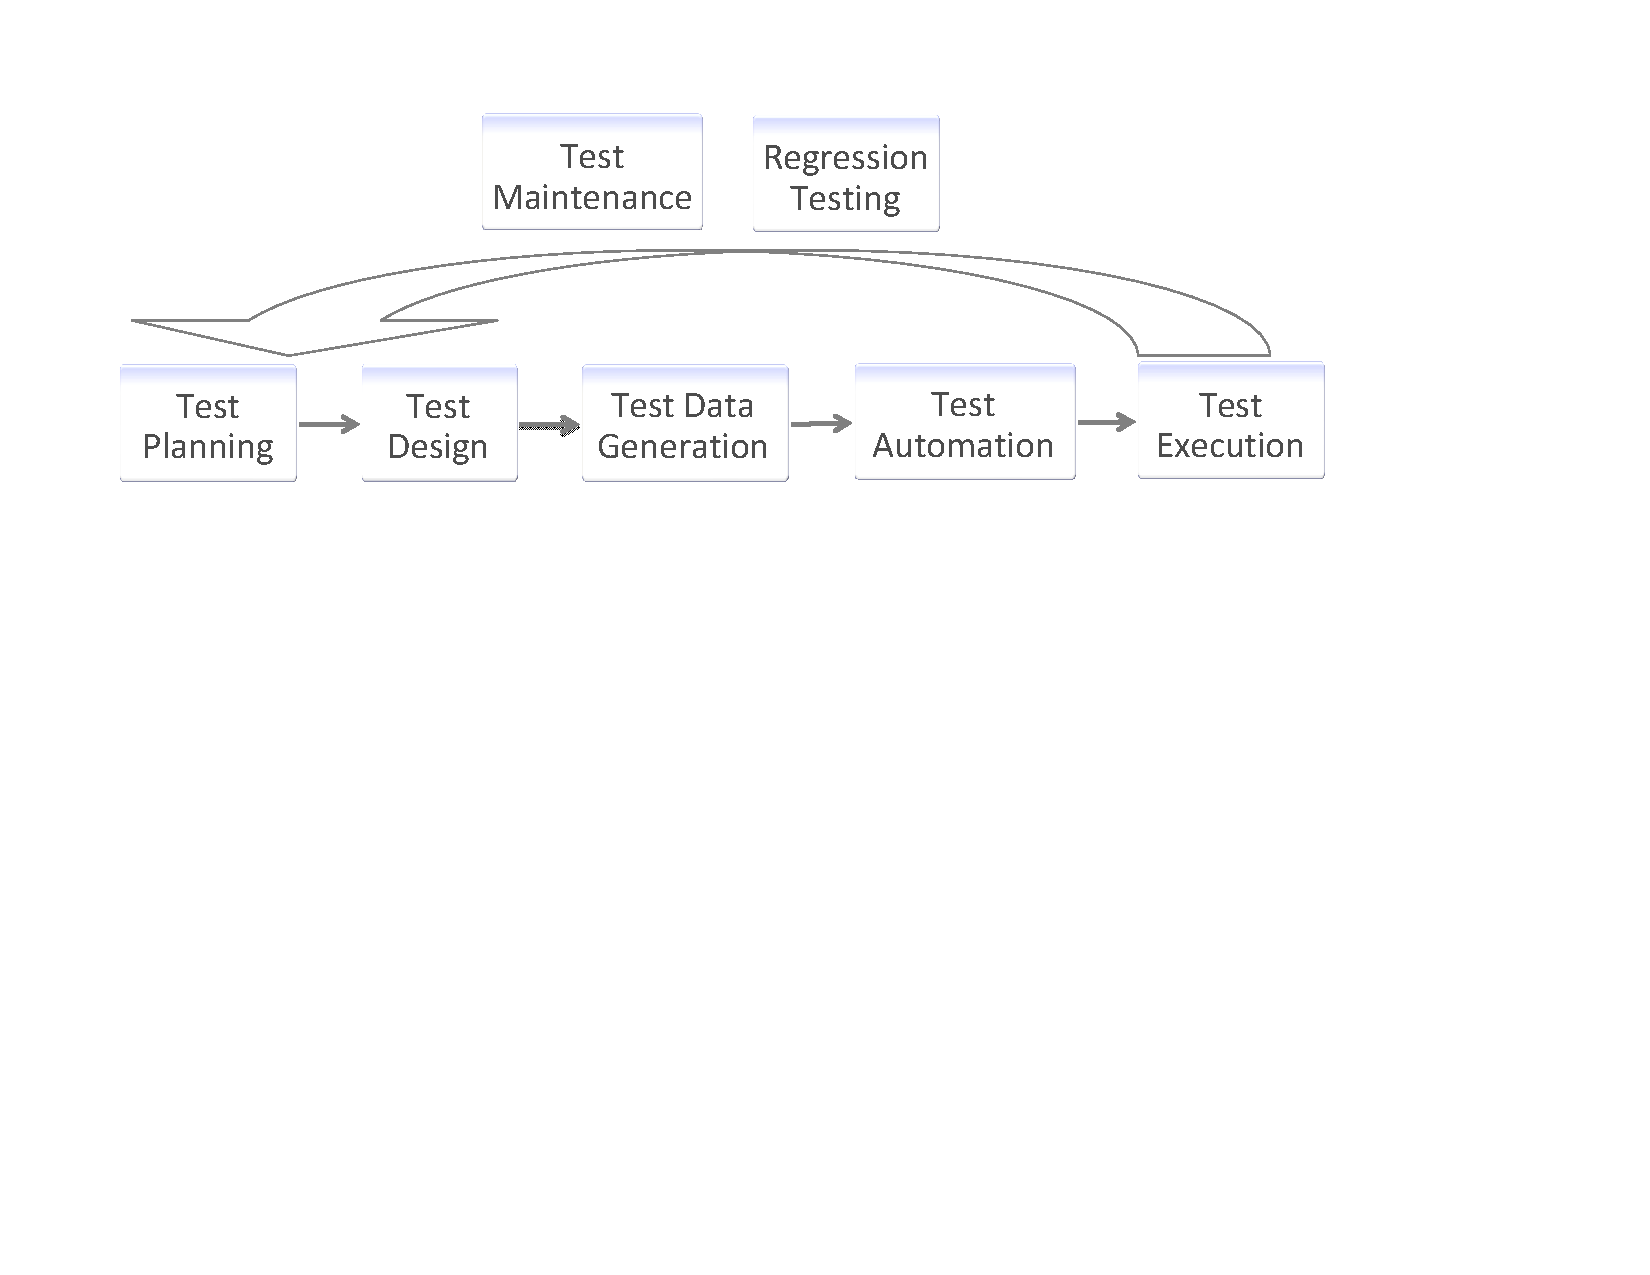
\includegraphics[width=\columnwidth, clip, trim = 22mm 133mm 65mm
  17mm]{figs/testing-activities.pdf}
\vspace*{-15pt}
\caption{Typical testing activities performed in delivery of testing services.}
\vspace*{-10pt}
\label{fig:testing-activities}
\end{figure}

The nature of the activities performed in a testing-services engagement can vary
from client to client. The scope of work can include any of test planning, test design,
test-data creation, test automation, test execution, and test maintenance. 
Figure~\ref{fig:testing-activities} presents an overview of
the commonly performed activities in testing services. 
A particular engagement might involve any subset of these activities; for example,
tesing for a client could involve only test execution, with the other
activities done by the client or by other vendors.  
%% The nature of
%% the test cases can also vary from functional tests to tests that focus on
%% validating non-functional system properties, such as performance and security.

%% The activities shown in Figure~\ref{fig:testing-activities}, of course, pertain
%% to testing in general (whether performed in-house or in an outsourced manner),
%% but there are factors that can add unique challenges in the setting of testing
%% services.  

Although software testing appears to be full of opportunities for automated tools,
for a variety of reasons, testing services remains largely a labor-intensive
business.  For example, manual testing of GUI-based applications is surprisingly
common, and testers routinely make up test data without methodical analysis.

Here are some of the reasons testing services is labor intensive.  First, the
automated techniques available today do not necessarily hold up to enterprise
applications, which include a heterogeneous mix of languages and technologies,
and for which requirements are written in prose by business analysts.  Second,
none of the techniques that require source code analysis or inspection are
typically applicable because the vendor offering testing services is given only
``black box'' access to the system under test.  Third, deliverables of testing
activity must be shown rather quickly (because revenues for the vendor are tied
to deliverables), and a long investment in time and money that is needed in
deployment of a tool is rarely tolerated either by the vendor or the client.  A
related reason is that the supply of labor that can deliver testing services has
hitherto been plentiful and affordable, reducing the economic motivation to
invest in tools.

The only ``testing'' tools that are routinely used in testing services are test
management and reporting tools that help keep track of the tests that have been
run (often manually) and their outcomes.

However, given the growth in testing services, it is inevitable that it needs to move from
a labor intensive business to an assets and tools-based business.  Therefore, 
research in this area is about automated tools so that 
testing can be carried out at lower cost and with consistent quality.  
Implicit in the abovementioned reasons is that the proposed solutions should be 
quick to deploy, low cost, and accessible to a large labor pool.

%%For instance, many of these activities can require specific skills in
%%testing techniques/tools or coding expertise, which the average testing
%%practitioner involved in service delivery may not possess. Second, some of the
%%activities may need to be carried out in strict time-bound cycles (governed by
%%service-level agreements) and in client-controlled test environments. Finally,
%%the myriad of technologies that must be accommodated in the contexts of the IT
%%systems of different clients adds another layer of complexity for service
%%companies.

%%Thus, in the setting of testing services, with its unique characteristics and
%%challenges, manual test creation, execution, and maintenance is still done quite
%%often.  The main goal of introducing innovation in this setting is to bring
%%automation and rigor to the testing tasks that are performed manually, sometimes
%%in an ad-hoc manner, and are prone to human lapses.

%%The testing research community has seen a long line of research (running into a
%%few decades) developing automated techniques for a variety of testing
%%problems---such as test-adequacy assessment, test-input generation, regression
%%test selection, test augmentation, test prioritization, and test
%%minimization---for imperative and object-oriented programs, and applicable to
%%different types of systems (\eg component-based systems and web
%%applications). For instance, there exists a large body of techniques for
%%automated test-input generation (\eg ~\cite{Artzi:2011, Boyapati:2002, cadar08,
%%  Clarke:1976, Ferguson:1996, godefroid05, Gross:2012, Harman:2010, king76jul,
%%  korel90aug, Pacheco:2007, sen05, thummalapenta:2011, Tillmann:2005,
%%  visser04}).  But, many of the techniques are inapplicable, or at least there
%%are significant challenges in applying them, in the context of testing
%%services. As already mentioned, most enterprise applications include a mix of
%%languages and technologies; thus, the automated techniques must deal with this
%%complexity. Second, in testing services, the vendor often does not have access
%%to the source code of the applications under test; thus, program-analysis-based
%%techniques would be inapplicable in these cases. Third, many automated
%%techniques---\eg much of the research on test-input generation---focus on unit
%%testing, which is not in the scope of work in testing services.

In the rest of this section, we discuss the testing activities shown in
Figure~\ref{fig:testing-activities}. For each activity, we present a sample of
relevant existing research and identify important unsolved (or partially solved)
problems for which the development of new automated techniques would make
valuable research contributions.

\subsection{Test Planning and Optimization}
\label{sec:test-planning}

Test planning involves tasks such as establishing the test process or strategy,
allocating resources, estimating cost and schedule, defining test-environment
requirements, identifying test targets, determining risk profiles for targets,
projecting defects and test numbers for each target, etc.  Test planning can be
done at multiple levels---such as macro planning at the start of a project which
evolves into micro planning as the project proceeds---and the test plan needs to
be continuously refined during the course of a project as more accurate
information becomes available.

\subsubsection*{Research Topic: ROI on Testing}

Test planning is intended not only to guide all downstream testing activities,
including test design, test execution, test-data and test-environment
provisioning, test reporting, etc., it should also answer key business
questions, such as~\cite{Kagan:NextGenTesting}

\begin{itemize}
\denseitems

%%\item How do we determine the quality of our testing effort?

\item Are we getting our money's worth out of testing?

\item Are we doing too much or too little testing?

\item Will an increased testing investment drive further improvement in quality?

%%\item Our testing budget was cut---what testing should we eliminate what will be
%%  its impact on product quality?

\end{itemize}

It has long been believed that more the testing, less the likelihood of defects
escaping to the field, and yet there is a point of diminishing return at which
it is no longer cost effective to invest in testing.  However, this judgment is
made mostly on intuition.  Little is available to managers by way of
quantititive techniques to balance the cost and benefit of continued testing.
Therefore, one of the research problems is to mine historical project data
across a number of projects to formulate techniques for balancing the cost of
testing with the return that it provides in terms of risk reduction.  Li and
Boehm~\cite{Li:2013} have recently presented an approach to prioritize tests
based on their business value.

%One of the challenges in test planning is standardizing and automating it, using
%data intelligence and forecasting. The availability of appropriate data is
%central to accurate forecasting and construction of prediction models (\eg for
%defect prediction). Although in a project, such data may be scarce initially, in
%the context of testing services, the vendor has the opportunity to mine and
%leverage data from hundreds of client projects to build benchmark data that can
%improve the accuracy of even the initial estimates in a project. This is another
%instance of the problem of capturing and leveraging organizational knowledge,
%across multiple client engagements, discussed in Section~\ref{sec:km}. In the
%context of test planning, we see further opportunities for research
%contributions in the types of data to be mined, anonymized, cataloged, linked,
%and organized for use in building accurate prediction models for testing-related
%activities.

\subsubsection*{Research Topic: Efficient Test Optimization}

In a testing-service engagement, a vendor can inherit existing test cases,
possibly designed by another vendor, for the applications under test. In fact,
in large testing-services engagements, the number of such test cases can easily
run into tens of thousands (sometimes even exceeding a couple of hundred
thousand).  To make matters worse, often, the test cases are captured in natural
language, stored in unstructured and varying formats (\eg in plain-text
documents or spreadsheets), and contain redundancies. 
%Thus, the vendor testing
%teams face the daunting task of taking stock of the available test cases,
%understanding them, and optimizing them.

Tools for extracting relevant information about test cases (\eg test name, test
steps, test prerequisites, expected outcome) from the diverse formats of
natural-language descriptions, and tools for clustering test cases (based on the
natural-language descriptions of tests) would be extremely valuable in assisting
testers in efficiently getting a good handle on a large corpora of unfamiliar
test cases. 
%Techniques from natural-language-processing and machine-learning
%communities can be profitably leveraged toward solving these problems.

Because it is generally infeasible to run such a large number of tests in each
regression cycle, testers must decide which tests to run---and despite the size,
a test suite may not give a balanced coverage of the application.  Thus,
techniques are needed to select test scenarios systematically.

One such technique---used extensively at IBM---is combinatorial test design
(CTD)~\cite{Cohen:1996, Cohen:1997, Cohen:2003}.  With CTD, first an
application's behavior is modeled in terms of key attributes, and the points of
variability of each attribute are determined. Then, an algorithm systematically
generates combinations of attribute-values that should be exercised.  CTD
manages combinatorial explosion in a principled way, \eg by testing only 
2-way combinations of attribute-values.  However, the use of CTD requires high
domain expertise and modeling skill, which is an inhibitor to its broad
adoption.  Effective tool support for simplifying model
construction~\cite{Segall:2012a}, iteratively refining
models~\cite{Segall:2012b}, and debugging models~\cite{Farchi:2013} is an active
area of research, with scope for more contributions, \eg in supporting model
maintenance and evolution.
%%Assuming that accurate CTD models can be created for a client system, a
Another challenging unsolved problem is how to map the output of CTD 
%(\ie a $k$-way covering array) 
to existing test cases. This is a very tedious task, almost completely manually
performed, for which tool support would be very valuable.

%Another task that testers have to perform is optimizing large test suites by
%removing redundant tests while ensuring good test diversity and
%coverage.\footnote{\small Test optimization can also be addressed at the
%  test-execution level, which we discuss in Section~\ref{sec:test-maintenance};
%  in this section, we focus on design-level optimization.} Combinatorial test
%design (CTD)~\cite{Cohen:1996, Cohen:1997, Cohen:2003} is a useful technique for
%performing such optimization that has been rigorously researched. Applying CTD
%in the context of testing services, with the available skill level and the
%effort that goes in creating CTD models for an unfamiliar system---by
%identifying attributes and values (or points of variability), and
%restrictions---can be challenging. Effective tool support for simplifying model
%construction~\cite{Segall:2012a}, iteratively refining
%models~\cite{Segall:2012b}, and debugging models~\cite{Farchi:2013} is an active
%area of research, with scope for more contributions, \eg in supporting model
%maintenance and evolution.



\subsection{Test Data Generation}
\label{sec:test-data}

\subsection{Test Data Generation}

Enterprise applications are typically database-oriented, in that they make queries over databases and the program flow depends on the data retrieved as a result of a query.  In order to test whether the application satisfies its requirements, sufficient amount of test data must be made available in the database. Consider, for example, a banking application, in which one of the requirement to exercise is that if a customer makes a certain fixed deposit, and the person is a senior citizen, and also holds a checking account in the bank, then an addition 0.25\% is paid as interest. To test that this situation is handled correctly in the application, there should exist a customer in the database such that his or her age qualifies the person as senior citizen and the person also has a checking account. Notice that typically, customer data and account data would be maintained in separate database tables. Typically business requirements are complex, and there need to be specific entries in multiple tables for a scenario to work out.

When a client gives a testing contract, the client may expect the service provider to exercise all the business rules, but may not give enough sample data in the database to be able to exercise these rules.  It then becomes the responsibility of the service provider to figure out the requisite test data to be present in the pertinent tables.

Randomly generated test data  cannot be expected to suffice for enterprise applications with complex rules. Also, systematic test generation approaches based on program analysis cannot be expected to tackle enterprise application, which use a mix of multiple language and database technologies in their implementation. The database community has done some work in creating test data for SQL queries, and that may be relevant; however, as mentioned before, enterprise applications are implemented with a mix of technologies.

We see a big opportunity for research contributions in this subarea. How to take a specification of the application as testing criteria, and automatically populate database that would enable various scenarios that fulfill the test criteria to be exercised.


\subsection{Test Automation}
\label{sec:test-automation}

The functional test cases for enterprise applications are often stated
informally in natural language. These tests are known as \textit{manual test
  cases}, which consist of a sequence of steps, intended for execution by a
human on the application user interface (UI).  Test automation is the activity
of converting these test cases into test scripts or programs that perform the
test steps mechanically. After creation, the automated test scripts can be
executed in regression cycles without any human intervention. For example,
Figure~\ref{fig:sample-test-case} shows a manual test case written in plain
English (left) and the corresponding tool-agnostic automated test script
(right). Typically, some amount of metadata necessary for locating the UI
elements is also stored in the test scripts.

\begin{figure}[t]
\centering
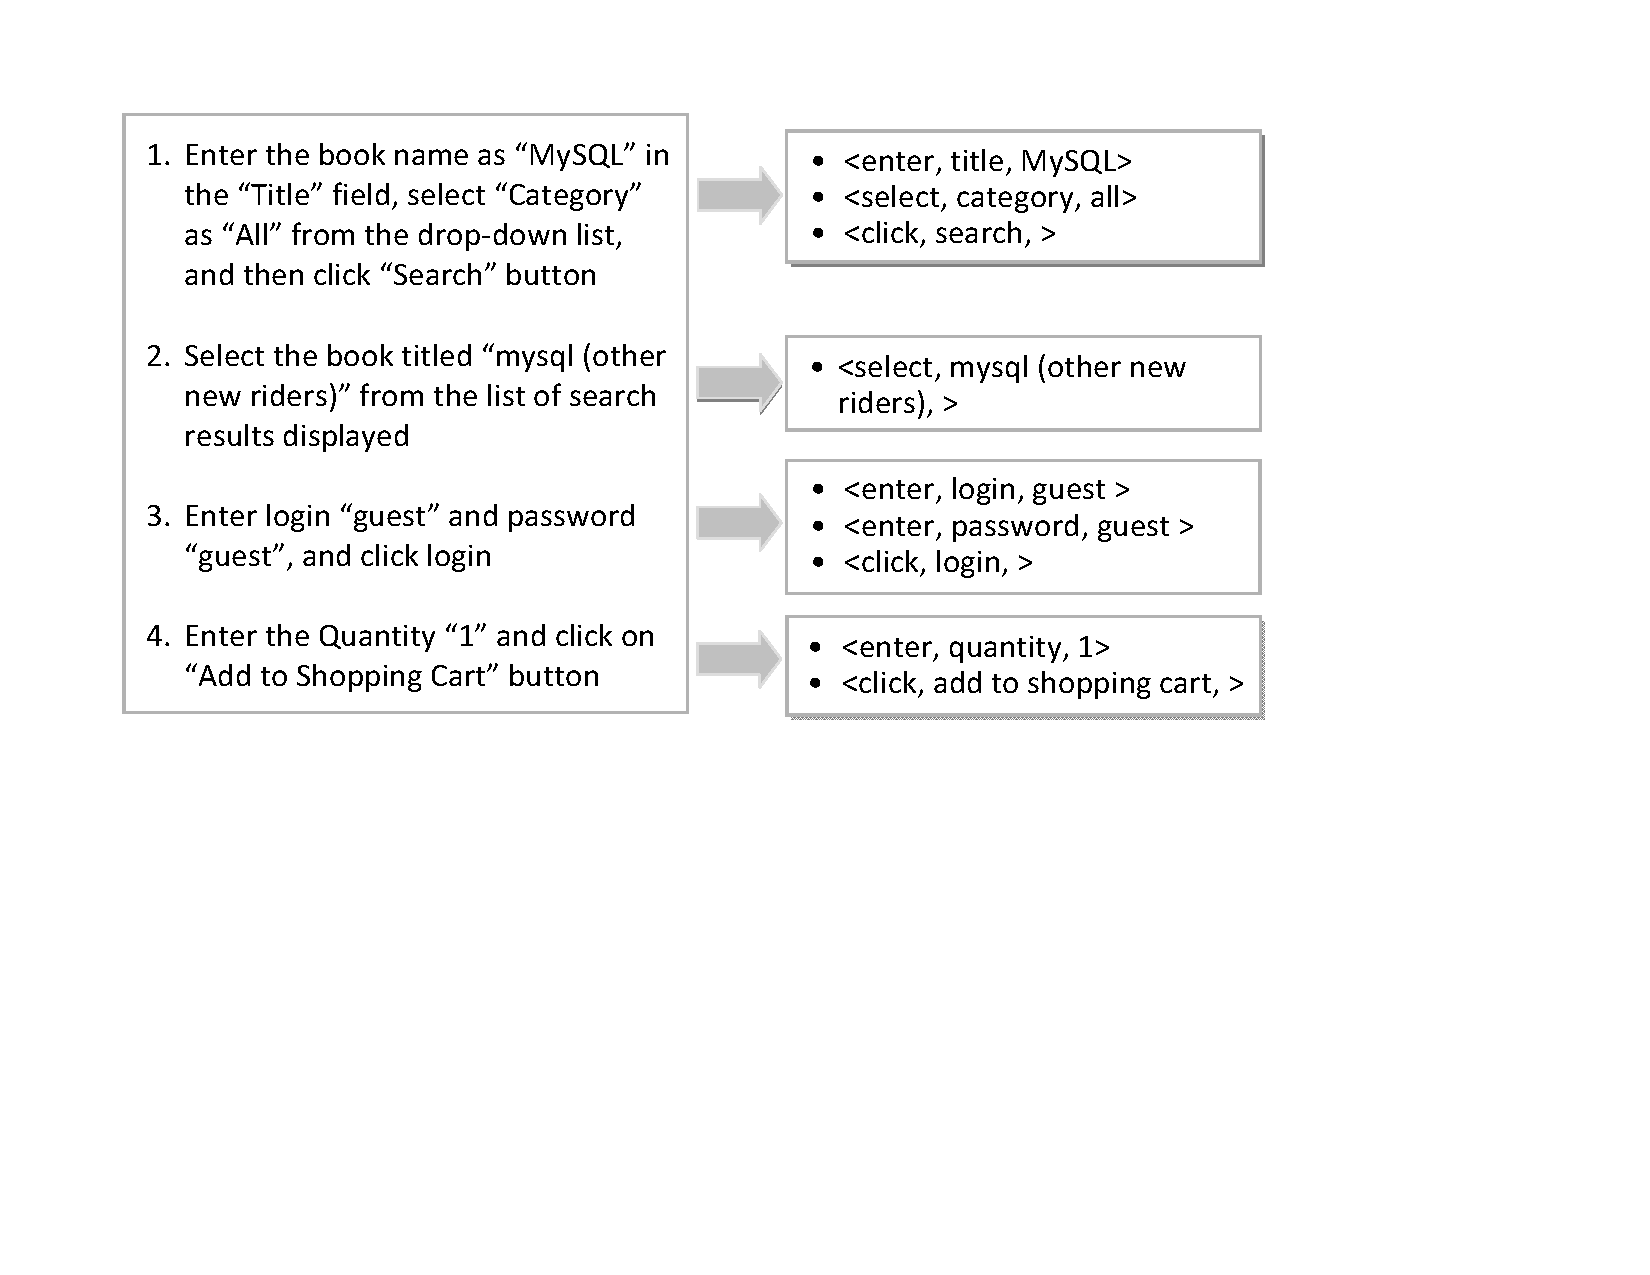
\includegraphics[width=\columnwidth, clip, trim = 21mm 93mm 65mm
  18mm]{figs/sample-test-case.pdf}
\vspace*{-15pt}
\caption{Sample manual test case and tool-agnostic script representation.}
\vspace*{-10pt}
\label{fig:sample-test-case}
\end{figure}

Although test automation is desirable (\eg for efficient and predictable test
executions) and sometimes necessary (\eg to meet time-constrained regression
schedules), creating \textit{robust} test scripts that can be used repeatedly in
regression cycles is expensive. In essence, creating such scripts is
time-consuming, involving a significant amount of coding, and requires expertise
in test automation tools (\eg \cite{hpqtp,ibmrft,selenium}). In the context of
testing services, this poses the unique challenge: how can change-resilient test
scripts be created efficiently by delivery personnel who may not possess good
programming skills or deep tool knowledge? 

%% Moreover, test automation involves not only the one-time cost of creating the
%% scripts, but also a recurring cost of maintaining the scripts in response to
%% application changes and changes in the execution environment.

\subsubsection*{Research Topic: Creating Robust Test Scripts}

The core problem that needs to be addressed in creating robust test scripts is
how to locate UI elements in a reliable manner. Moreover, there are different
dimensions along which this problem needs to be investigated: the need for
executing test scripts on different platforms, execution environments, or
application variants. We discuss both these aspects of script robustness.

\vskip -5pt
\paragraph*{Locating UI Elements Reliably} In general, there are two broad categories of
techniques for locating UI elements. The first category relies on the structure
of the internal representation of the UI
%% ~\footnote{\small In the context of web applications, the internal UI
%%   representation is the Document Object Model (DOM).}
and on internal attributes, such as IDs or names, of UI elements/widgets. Sample
test-automation tools in this category include IBM Rational Functional
Tester~\cite{ibmrft}, HP QuickTest Professional (QTP)~\cite{hpqtp}, and
Selenium~\cite{selenium}. Over-reliance on internal structures and attributes
can make scripts fragile (\eg if the structure changes often or the attributes
are generated dynamically).
%% and, in particular, unreliable for execution across
%% browsers and platforms.

The second category of tools rely on image processing to locate UI elements;
sample tools in this space include Eggplant~\cite{Eggplant} and
Sikuli~\cite{Chang:2010, Yeh:2009}. These tools record a test script as a
sequence of actions performed on images. During automation, the tester grabs a
portion of the screen around the element of interest, specifies the coordinates
in the selected region where the action is to be performed, and specifies the
image-similarity threshold to be to locate the element. By being independent of
internal structure and attributes, such tools are resilient to changes in the
internal structure/attributes, but they are fragile in the presence of
differences in visual rendering. %%, say across browsers or application variants.

A third, and less-common, alternative to these approaches is to associate with a
UI element a label in the vicinity of that element, and refer to the element via
its associated label. This approach, which is used in the \textsc{ata} tool
developed at IBM~\cite{thummalapenta:2012b, thummalapenta:2012a,
  thummalapenta:2013a} and also supported by QTP~\cite{hpqtp}, can overcome the
limitations of approaches that rely on internal structure or image
processing. But, the currently available implementations of these approaches
perform simple label associations (based on visual proximity only) and are
inapplicable when ambiguous labels exist. Development of more powerful and
generally applicable techniques for label association would be a fruitful
direction of research.

These approaches have different strengths and weaknesses; it is quite possible
that no one approach turns out to be the best in all circumstances. For example,
an image-based technique may outperform an internal-structure-based technique
for cross-browser test execution; but, the converse would likely be true for
test execution across locale-specific versions of a web application. In
practice, the choice of the technique would have to be tailored to the
requirements of testing.  Development of tools that combine the approaches, and
rigorous empirical studies that evaluate the resiliency of these approaches for
different types of testing would make valuable research contributions.

\vskip -5pt
\paragraph*{Test Portability across Platforms} The second aspect of script robustness is the
challenge of executing automated test scripts on different platforms, execution
environments, or application variants.  For example, functional testing of web
applications needs to be performed on different browsers to detect potential
cross-browser incompatibility
defects~\cite{Choudhary2010,Shauvik:2012,Choudhary:2013,Mesbah:2011}. Ideally,
in such situations, a test script should be agnostic to browser-specific
differences unless, of course, those differences are symptoms of application
defects.

Similarly, in the context of mobile applications, test automation faces the
formidable challenge of high diversity: many platforms, devices, web browsers,
and application variants. For instance a mobile application can have native,
hybrid, and web variants, with different platform-specific native variants. In
the face of such enormous diversity, to what extent can a script automated on
one platform/variant be executed on another platform variant with automated
adaptation?  In cases where the UI layout and flow is exactly the same across
application variants, a test script recorded in a platform-agnostic script
notation (\eg \cite{PerfectoScriptOnce}) on one variant can be executed, without
modification, on another variant.  But, in more complicated cases, the UI layout
and flow for the same scenario may differ across variants.

%Recent work on mobile application testing has focused on recovering state models
%via random and/or directed application crawling, and using the state models to
%generate test cases systematically (\eg \cite{Amalfitano:2011, Amalfitano:2012,
%  Choi:2013, Hu:2011, Joorabchi:2012, Yang:2013}). Symbolic-execution-based
%approaches for test generation are also being investigated~\cite{Anand:2012,
%  Mirzaei:2012}. The problem of automated test adaptation across application
%variants has not yet been investigated but, if suitable techniques are
%developed, they could be useful generally and more so in the context of testing
%services.

%In testing services, the problem of test adaptation also shows up in the context
%of packaged applications, such as SAP. Typically, the implementation of a
%packaged application for a client requires the customization of default data
%definitions, processes, user interfaces, etc. to the client's requirements. Such
%customizations modify the default flows available through the application UI,
%raising the question of whether test scripts can be automatically adapted to
%accommodate the changes.

%We believe there is scope for the development of advanced techniques that
%perform such test adaptation, across platforms, variants, and cutomizations,
%while ensuring that the intent of the test cases are preserved.

\subsubsection*{Research Topic: Automated Test-Script Synthesis}

The problem of converting manual test cases to automated test scripts can be
looked upon as an instance of program synthesis~\cite{Gulwani:2010}.  Program
synthesis addresses the problem of discovering a program that realizes a given
user intent. There are three dimensions of the synthesis problem: the form of
user intent, the search space of programs, and the search
technique~\cite{Gulwani:2010}. For instance, the user intent could be stated in
different forms such as, natural language, input-output examples, logical
relations between inputs and outputs, and demonstrations. In test automation,
user intent is specified in the form of manual test steps, and the end goal is
an automated script that realizes that intent (\eg as shown in
Figure~\ref{fig:sample-test-case}).

Recent work~\cite{thummalapenta:2012a} has attempted to automate the creation of
test scripts from manual test steps by combining natural-language processing
with dynamic exploration of multiple flows, via backtracking, to search for the
correct test script from the space of possible scripts. However, there are
practical limitations of that technique: dynamic exploration of alternative
flows via the application UI can encounter problems such as persistent state
updates during an exploration that may have to be undone or disabled UI elements
that limit the scope of exploration. Addressing these problems is important for
effective exploration of the space of possible test scripts.

Type-based program synthesis~\cite{Perelman:2012} and natural-language
processing have also been applied for creating automation scripts for
smartphones from natural-language descriptions of tasks~\cite{Le:2013}. Such
approaches could also be leveraged for test automation. Creation of test scripts
can often require the coding of custom functions; for example, a verification
step in a test might require checking that the values in a drop-down list are
sorted or that some value exists in a particular cell of a table. Currently,
such code must be written manually. Automatic synthesis of such code, based on a
specification of user intent, could go a long way in automating the overall
creation of test scripts.

\subsection{Test Maintenance}
\label{sec:test-maintenance}

As an application evolves and its test suite grows in size, the suite can
require maintenance to remove obsolete tests, repair broken tests, and eliminate
any redundancies~\cite{Pinto:2012}.  Application evolution can occur in response
to changed requirements or business rules, or it could occur in the form of code
refactoring. In either case, these pose challenges in keeping a test suite
up-to-date.

\subsubsection*{Research Topic: Identifying Obsolete Tests}

When an application is modified to accommodate changed requirements, it can be
hard to identify which test cases have become obsolete.  In general, a test
failure observed on a new version of the application can either expose
application faults or result from a problem with the test itself. Determining
this reason for failure is the critical first step before any corrective action
can be taken---repairing the test if the test is broken, or fixing the
application if the test has revealed an application fault. Without any tool
assistance and faced with a large number of test failures, testers can tend
toward ignoring test-execution results or, even worse, deleting failing tests,
which can quickly degrade test-suite coverage and defeat the purpose of testing.

Researchers are starting to address the problem of automatically identifying
obsolete tests---\eg Reference~\cite{Hao:2013} presents a machine-learning-based
approach for separating obsolete tests from application bugs in the context of
unit testing---but these are only initial results on this topic. The development
of more powerful techniques that possibly take into account changes in
specifications and that are more generally applicable (\eg for system-level GUI
tests) is a challenging but promising research direction.

\subsubsection*{Research Topic: Automated Test-Flow Repair}

If a failure results from a broken test, the test needs to be repaired.  For
example, refactoring of the application GUI, such as splitting a web page into
multiple tabbed pages, can break the flow of a test~\cite{thummalapenta:2013a},
which would occur irrespective of how robust the mechanism for locating UI
elements is. Such changes require the test flow to be repaired, involving
addition or deletion of test steps---automatically performing such repairs is
beyond the capability many of existing GUI test repair
techniques~\cite{Choudhary:2011, Grechanik:2009, Memon:2008}.

Automated test-repair techniques have also been developed for unit
tests~\cite{Daniel:2009, Daniel:2010, Mirzaaghaei:2012}, but they are not
relevant in the setting of testing services for a couple of reasons pointed out
earlier: unit testing is typically not in the scope of activities to be
performed and program-analysis-based techniques are usually inapplicable.

%% The problem of test-flow repair is similar to the problem of test adaptation
%% across platforms and application variants, but there are differences that can
%% influence the types of techniques that can be developed. In the case of
%% test-flow repair, two \textit{versions} of the same application are available
%% along with change information captured in version-management systems. Thus,
%% static program-differencing techniques and analysis of change logs could be
%% leveraged to guide flow repair. In contrast, for test adaptation across
%% platforms, two \textit{variants} of the application, implemented in different
%% programming languages (\eg Objective-C for iOS variants and Java for Android
%% variants), would be available; thus, static-analysis techniques may not be
%% readily applicable.

Proposals for GUI-refactoring-driven test repair~\cite{Daniel2011} accommodate
certain types of GUI refactorings (\eg replacing a radio box with a drop-down
list), but do not as yet address general flow repair.  Recent research has seen
the development of repair techniques for broken GUI flows~\cite{Zhang2013},
addressing some of the limitations of the existing test-repair techniques, but
there are opportunities for more research contributions on this topic---\eg
through further investigation of techniques that combine static program analysis
and dynamic GUI exploration.

\subsubsection*{Research Topic: Reducing Redundancies in Test Scripts}

Test scripts are software artifacts, and like other software artifacts, need to
be refactored occasionally.  Procedural abstraction means identifying common and
frequently occurring sequences of steps that can be extracted out as a
subroutine; \eg the steps required to log in into a web site can be extracted
out into a login subroutine~\cite{Mahmud:2010}.  Opportunities for procedural
abstraction arise in test scripts, among other reasons, due to rampant
cut-and-paste practices.  Refactoring makes a test suite easier to understand,
and easier to maintain going forward.  Somewhat unexpectedly, it can sometimes
also help reduce the execution time of a test suite---\eg Devaki et
al.~\cite{Devaki:2013} articulate criteria for merging multiple tests into one
without loss of coverage.

Further investigation of such techniques for improving test suites, that also
preserve fault-detection capability and are evolution-aware, can be a fruitful
research direction.

%Over time, as a suite of automated test scripts evolves, subtle redundancies can
%creep into it in the form of similar tests. Similar tests are not redundant by
%any measure; but, they contain many common actions that are executed repeatedly,
%which over a large test suite, can degrade execution time substantially.
%Sometimes, a service provider can inherit such test suites from another vendor,
%that have significant opportunities for optimization of test execution.

%Recent work on the idea of merging similar tests to improve test execution time,
%while preserving the fault-detection capability of the original test suite, has
%shown promising initial results~\cite{Devaki:2013}. But, such techniques need
%further development and evaluation. For instance, test merging must take into
%account application evolution because changes in the application can invalidate
%some of the merging performed on the old application version. (This problem
%afflicts, in general, all techniques for test-suite reduction.)  Development of
%scalable and efficient techniques for automated test merging, that preserve
%fault-detection capability and are evolution-aware, can be a fruitful research
%direction.


\section{Experiences}

Over the past few years, we have worked extensively on taking research
innovations from the lab to real-world deployment in IBM Global Business
Services. In this section, we highlight some of our experiences.

First of all, there is a fundamental tension between client expectation of the
service provider being bold and innovative, and at the same time provide
predictable, consistent delivery.  When vendors bid for a contract, the client
does want the vendor to bring innovation to impact both cost and quality. Once
the project gets going, however, the ground level realities of consistent
delivery must be met, and therefore project managers in charge of delivery need
to be conservative in their approach.

Any new process or tool causes at least a minor disruption in normal flow of
the project, and this makes pushing either a new process or a new tool into
project delivery significantly harder.  To compound matters, a project may move
from one vendor to another vendor for various reasons, and for this reason, the
client may not want to deviate from ``industry standard'' processes and tools,
because it would be difficult to back out of any thing experimental. Clients
often prohibit vendors from installing additional software in their IT
environment.

The second challenge occurs when a client already has an in-house tool in the
same space as the innovative tool being introduced by the vendor. In such cases,
displacing the incumbent tool based on merits of improved productivity or lower
cost is hard: the client would have the natural inclination to prefer their tool
over a potential lock-in with the vendor-proprietary tool whose stability in
their IT environment is yet to be proven.

The third issue in deploying an innovative tool is that it must solve the
problem that it is targeted for in a holistic manner in the client's application
landscape. For instance, consider an innovative test-automation tool that has
shown the promise of tremendous productivity improvement and lower costs over
conventional test-automation tools, but that is applicable to web applications
only. A client whose application portfolio includes a mix of web, mainframe, and
packaged applications, might appreciate the tool's many benefits, but would
still be reluctant to adopt it because it addresses the automation problem for
only part of their application portfolio.

The fourth challenge, which we also alluded to in the Introduction, is that
convincing clients of an innovative tool's benefits requires immersive
demonstrations over and over again. Often a client requires multiple
demonstrations and even proof-of-concepts in their IT environment and on their
artifacts, and integration with their existing tool chain. Thus, rolling out an
innovation for the next client might require as much work as it did for the
previous client.

The fifth challenge is that the skill levels of the practitioners vary widely
and, moreover, business pressures often require them to move from project to
project. In such a scenario, getting practitioners to enthusiastically learn new
tools is difficult.  Moreover, tools in which there is no immediate reward to
them---\eg entering information in a knowledge management system---are even
harder to get adopted.

The final challenge is that services companies are not equipped to curate
software tools in house. Thus, a tool developed in the lab, even when it proves
its value, sometimes meets with difficulties because there is no organization to
``own'' and support the tool for long periods of time. In the long term, the
tool can neither stay in the lab nor move, and be owned, outside of it,
heralding its eventual obsolence.

The research challenge is to design tools in a way that are (1)~minimally
disruptive and (2) easy to learn. Incentivization schemes, also known as
gameification, are an exciting area of research with tremendous implications on
service delivery.  Open sourcing may be a way to get tools to be supported in
the community for a long time, though this obviously is at odds with the
vendor's desire to have exclusive, differentiating technology.


\section{Conclusion}
\label{sec:conclusion}

Software services companies rely crucially innovations in individual and
organizations productivity for their competitiveness. In this paper, we examined
some of the topics that require attention from the software engineering research
community. We examined challenges in how modern services companies organize
their work and workforce; challenges in knowledge management at an organization
level; issues in risk assessment; and finally challenges in testing services. We
also discusses challenges in deployment of research innovations in real-world
services context. We hope that the research community takes a careful look at
the software services industry for many opportunities for impact.

\section*{Acknowledgements}
The research agenda presented in this paper is a collation of knowledge the
authors and various other IBM Researchers accumulated in course of working with
IBM's service delivery practitioners. From services delivery, we would like to
thank Anup K Ghosh, Jack Bisceglia, and Achin K Das for sharing the IT delivery
challenges and championing the use of research tools in their teams. At IBM
Research, we would like to thank Sugata Ghosal, Manish Gupta, and Rakesh Mohan
for driving the services delivery research agenda. We would also like to
acknowledge our colleagues Min Chee, Pankaj Dhoolia, Richard Goodwin, Juhnyoung
Lee, Debapriyo Majumdar, Senthil Mani, Pietro Mazzoleni, Debdoot Muk\-herjee,
Diptikalyan Saha, Karthik Sankaranarayanan, Bikram Sengupta, Renuka Sindhgatta,
Suresh Thummalapenta, and Joe Zhou, who have been involved in various research
initiatives during course of which the challenges listed in this paper were
identified.

\bibliographystyle{abbrvnat}
{\small
%\balance
\bibliography{fose,risk-global,km}
}

\end{document}
